\documentclass[14pt, oneside]{altsu-bachelor}

\title{Цифровой генератор сигналов на основе микроконтроллера STM32}
\author{Д.\,С.~Вебер}
\groupnumber{506}
\GradebookNumber{294}
\supervisor{П.\,Н.~Уланов}
\supervisordegree{ст. преп.}
\ministry{Министерство науки и высшего образования}
\country{Российской Федерации}
\fulluniversityname{ФГБОУ ВО Алтайский государственный университет}
\institute{Институт цифровых технологий, электроники и физики}
\department{Кафедра вычислительной техники и электроники}
\departmentchief{В.\,В.~Пашнев}
\departmentchiefdegree{к.ф.-м.н., доцент}
\shortdepartment{ВТиЭ}
\ChairmanOfTheStateCertificationCommission{С.\,П.~Пронин}
\ChairmanOfTheStateCertificationCommissiondegree{д.т.н., проф.}
\NormController{А.\,В.~Калачёв}
\NormControllerdegree{к.ф.-м.н., доцент}
\Consultant{}
\Consultantdegree{}
\UDC{519.688}
\docname{БР 09.03.01}
\abstractRU
{
В первой главе были рассмотрены семейства микроконтроллеров, различные среды разработки и изучены методы программной генерации сигналов.

Во второй главе был спроектирован генератор. Проведено моделирование выбранного метода генерации, разработан алгоритм работы и создана схема электрическая принципиальная.

В третьей главе была произведена сборка макета, написана и протестирована результирующая программа. 
}
%\abstractEN
%{
%In the first chapter, families of microcontrollers, various development environments were considered and methods of software signal generation were studied.

%In the second chapter, a generator was designed. The simulation of the selected generation method was carried out, an algorithm of operation was developed and an electrical circuit was created.

%In the third chapter, the layout was assembled, the resulting program was written and tested.
%}
\keysRU{генератор сигналов, микроконтроллер}
\keysEN{signal generator, microcontroller}

\date{\the\year}

% Подключение файлов с библиотекой.
\addbibresource{graduate-students.bib}

\begin{document}
\maketitle

\setcounter{page}{2}
\makeabstract
\tableofcontents

\chapter*{ВВЕДЕНИЕ}
\addcontentsline{toc}{chapter}{Введение}
%нужно зайти из далека для настройки калибровки радио 
	В ходе эксплуатации электронных устройств регулярно возникает необходимость в настройке или ремонте. Для калибровки и отладки приборов необходимы колебания разных форм и периодов. Формирование требуемых электрических колебаний может обеспечить специализированное устройство --- генератор сигналов.
	
	Генератор сигналов --- это неотъемлемый инструмент для любого специалиста в области электроники. %У многих специалистов есть необходимость без применения дорогостоящих средств генерировать колебания с установленными параметрами. 
	На сегодняшний день разрабатывается достаточно много генераторов сигналов, % которые используются для различных исследований или необходимы для настройки каких-либо устройств,
	 но не все генераторы, которые есть на рынке, обладают компактными размерами, лёгкостью транспортировки и доступностью в цене. %Существует два основных вида генераторов --- аналоговый и цифровой.%
	
	Ранее практически все лабораторные генераторы были аналоговыми и конструировались на различных схемах. К их достоинствам можно отнести простоту и надёжность, но у них есть существенные недостатки в виде меньшей стабильности и более тщательной настройке. Сейчас практически все генераторы, которые есть на рынке создаются на основе цифровых методов синтеза аналоговых сигналов, %Цифровые генераторы легко интегрируются с другими системами и могут управляться через программное обеспечение, что упрощает процесс.%
	 т. к. они стабильные и точные. %., а также могут быть реализованы просто на микроконтроллере. 
	 Такого рода генераторы могут найти применение и в промышленности, но не всем пользователям требуются такие высокие характеристики. Разработанный в данной работе генератор претендует на применение в домашней лаборатории в качестве простого и функционального дешёвого генератора сигналов.
	
	Применением такого генератора может быть генерация сигналов разных форм, работа с аналоговыми системами для исследования влияния сигналов на них, изучение методов обработки сигнала или основ электроники. 
	
\textbf{Цель}
	выпускной квалификационной работы состоит в разработке цифрового генератора сигналов на микроконтроллере.

\textbf{Задачи}

	\begin{enumerate}
		\item Исследовать методы генерации сигналов и осуществить выбор.
		\item Рассмотреть семейства микроконтроллеров и осуществить выбор.
		\item Выбрать среду разработки.
		\item Разработать программу.
		\item Сконструировать макет.
		\item Протестировать генератор.
	\end{enumerate}

\chapter{Начало разработки}

\section{Обзор микроконтроллеров}



\section{Среды разработки для STM32}




\section{Методы программной генерации сигнала}
	Основные методы цифровой генерации сигналов --- метод аппроксимации и табличный метод.
	
	Метод аппроксимации подразумевает собой вычисление отсчётов функции с заданным интервалом. В памяти хранятся только параметры сигнала. Поэтому данный метод позволяет затратить небольшой объём памяти, но его недостаток это затраты на вычисления, что ограничивает максимальную частоту сигнала.
	
	В табличном методе генерации сигналов предполагается, что заранее вычисленные отсчёты хранятся в памяти. То есть никаких вычислений не требуется и генерация сводится к тому, что в порт цифро-аналогового преобразователя нужно вывести ячейку по заданному адресу. Таким образом, время на формирование отсчёта становится меньше и появляется возможность генерировать сигнал с более высокой частотой. Недостатком же является большие затраты памяти.
	
	Будем рассматривать табличный метод синтеза. Для начала потребуется таблица отсчётов, чтобы её вычислить используем готовый инструмент.
	
	\begin{figure}[H]
    \centering
    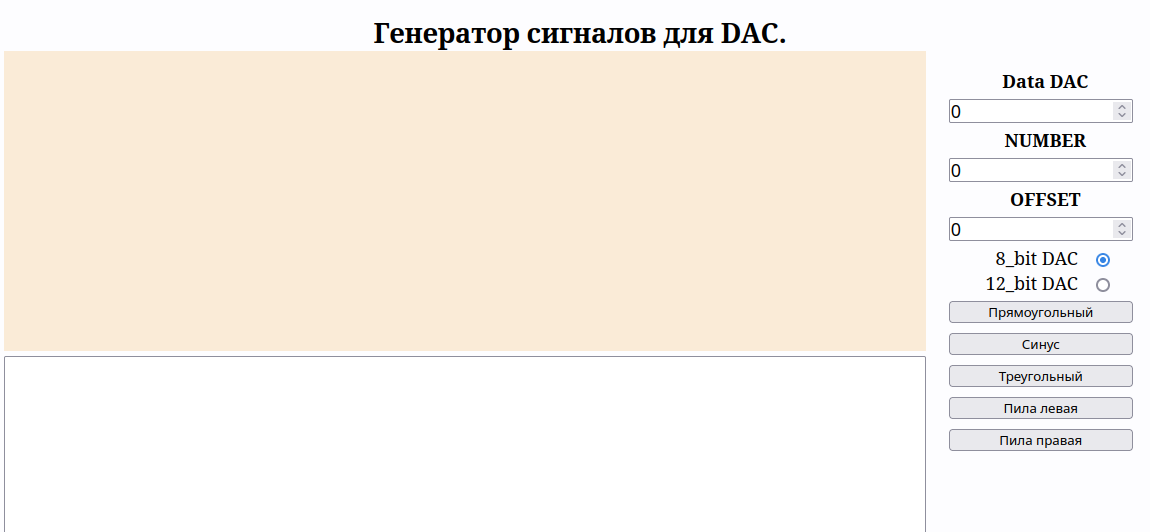
\includegraphics[width=1\textwidth]{../image/lut_prog.png}
    \caption{Программа для вычисления значений сигнала.}
	\end{figure}
	
	У таблицы есть 4 параметра:
	\begin{enumerate}
		\item Разрядность ЦАП: 8 или 12 бит.
		\item Максимальное значение.
		\item Количество значений.
		\item Смещение от нуля.
	\end{enumerate}
	
	Использовать мы будем 12-битные значения в количестве 256 чисел. Максимальное значение амплитуды сигнала может быть 4095, но так как для улучшения генерации будет задействован встроенный в цифро-аналоговый преобразователь выходной буфер, то он будет срезать сигнал сверху и снизу на 0.2В, поэтому значения тоже следует срезать на эту же величину для корректной генерации.
	
	В документе от ST про работу с цифро-аналоговым преобразователем есть формула для расчета выходного напряжения.
	
	$DAC_{output} = V_{REF}*\dfrac{DOR}{DAC_{MaxDigitalValue} + 1}$, где DOR --- цифровое значение.
	
	Нам нужно найти какое значение соответствует напряжению 0.2В. Выразим DOR и подставим имеющиеся значения.
	
	$DOR = \dfrac{3.3}{0.2}*(4095+1) = 248$
	
	Укажем смещение от нуля 248, а максимальное значение 4095 меньше на 248, то есть 3847 и сгенеририуем таблицу отсчётов для синусоиды. 
	
	\begin{figure}[H]
    \centering
    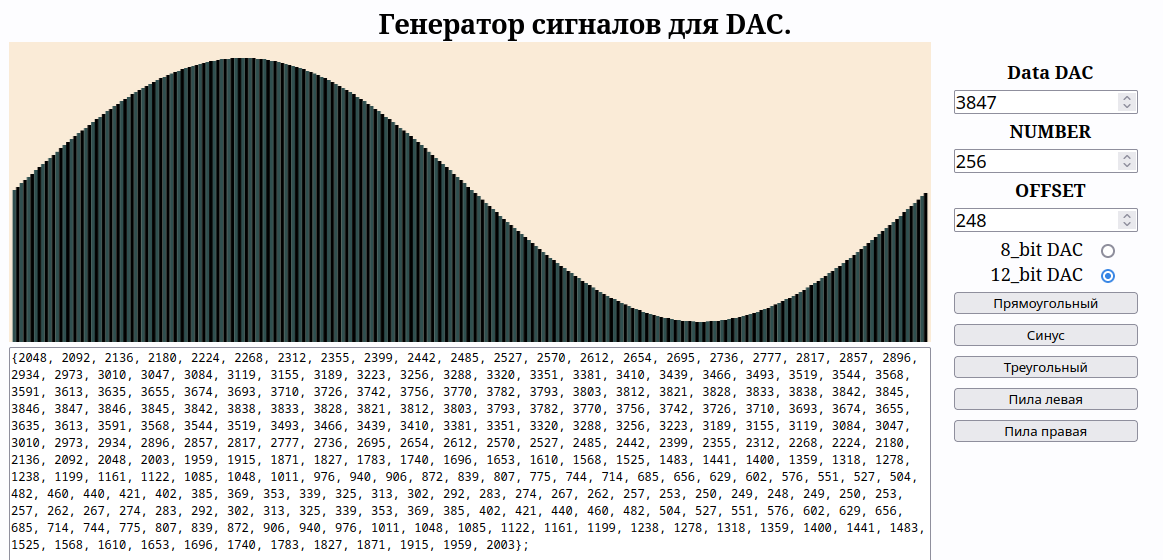
\includegraphics[width=1\textwidth]{../image/lut.png}
    \caption{Вычисление таблицы сигнала.}
	\end{figure}
	
	Теперь у нас есть данные для генерации сигнала, но теперь нужно продумать как передавать их в цап и как вообще работать с цапом.
\chapter{РАЗРАБОТКА ПРОГРАММЫ ДЛЯ ГЕНЕРАЦИИ СИГНАЛОВ}
\section{Моделирование DDS}
	Для начала потребуется таблица отсчётов, чтобы её вычислить используем готовый инструмент~\cite{lut}.
	
%	\begin{figure}[H]
%    \centering
%    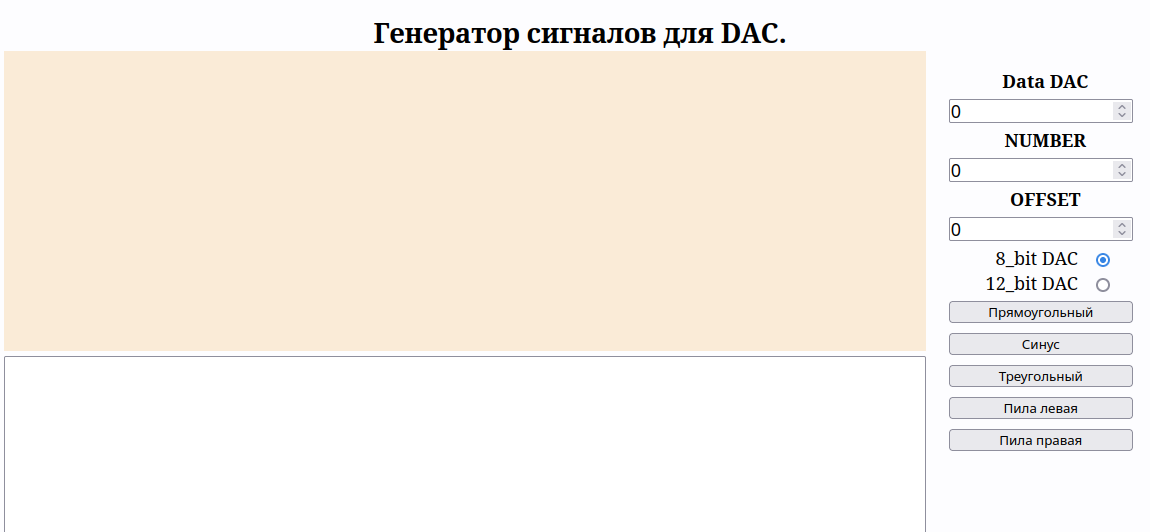
\includegraphics[width=1\textwidth]{../image/lut_prog.png}
%    \caption{Программа для вычисления значений сигнала.}
%	\end{figure}
	
	У таблицы есть 5 параметров:
	\begin{enumerate}
		\item Максимальное значение;
		\item Количество значений;
		\item Смещение от нуля;
		\item Разрядность ЦАП: 8 или 12 бит;
		\item Форма сигнала.
	\end{enumerate}
	
	В данной работе будут использоваться 12-битные значения в количестве 256 чисел. Максимальное значение амплитуды сигнала может быть 4095. Для примера вычислим таблицу значений для синусоиды.
	
	\begin{figure}[H]
    \centering
    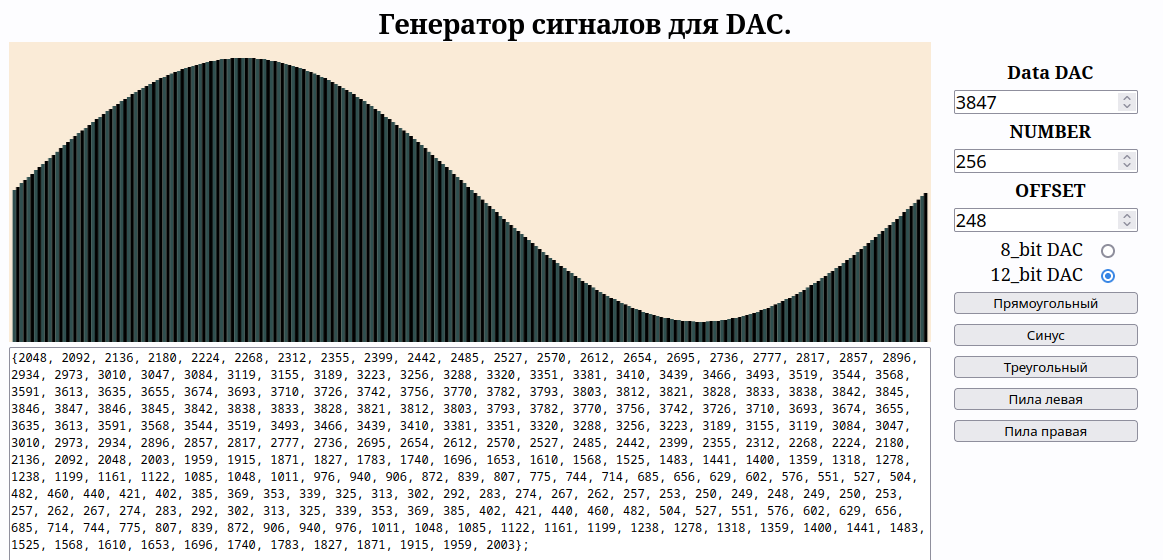
\includegraphics[width=1\textwidth]{../image/lut.png}
    \caption{Вычисление таблицы сигнала.}
	\end{figure}
	
	Теперь у нас есть данные для генерации сигнала. Смоделируем алгоритм метода прямого цифрового синтеза по блок-схеме на рис. 1.15 на языке Си для дальнейшей реализации на микроконтроллере.

\begin{code}
\captionof{listing}{Метод DDS}
\begin{minted}[mathescape,linenos,frame=lines,breaklines]{text}
int main() {
  uint16_t p_acc, p_step;
  uint8_t addr = 0; // адрес ячейки

  p_acc = 0;    // аккумулятор фазы
  p_step = 128; // код частоты

  while(1) {
    addr = p_acc >> 8; // выделение старшей части аккумулятора фазы
    p_acc += p_step;   // шаг
    printf("%d 0x%X\n", addr, sinus[addr]); // вывод отсчёта
  }

  return 0;
}
\end{minted}
\end{code}

	
	Код частоты задаёт выходную частоту генератора. При значении 256 вывод будет следующий:
	
\begin{figure}[H]
    \centering
    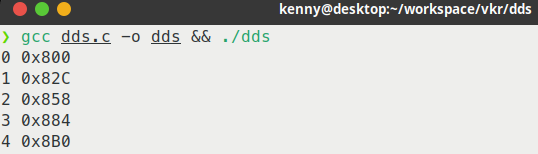
\includegraphics[width=0.6\textwidth]{../image/dds256.png}
    \caption{Формирование отсчётов при коде частоты 256.}
\end{figure}
	
	Увеличим код частоты в два раза и получим следующее:

\begin{figure}[H]
    \centering
    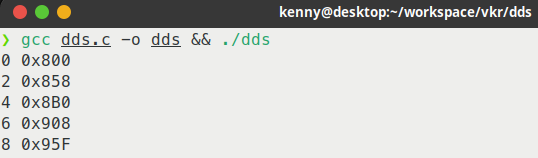
\includegraphics[width=0.6\textwidth]{../image/dds512.png}
    \caption{Формирование отсчётов при коде частоты 512.}
\end{figure}

	Как можно заметить отсчёты стали формироваться через один, соответственно частота вырастит в два раза. Теперь уменьшим частоту в два раза выставив код частоты 128.

\begin{figure}[H]
    \centering
    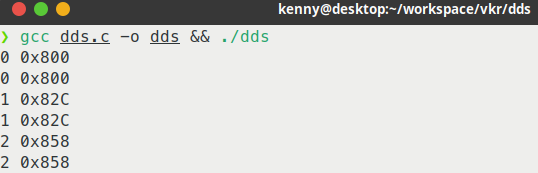
\includegraphics[width=0.6\textwidth]{../image/dds128.png}
    \caption{Формирование отсчётов при коде частоты 128.}
\end{figure}

	Программа стала выводить каждый отсчёт по два раза тем самым, понизив частоту.
	
	В данном виде модуляции код частоты просто абстрактное число, которое добавляется к аккумулятору фазы и узнать реальную частоту проблематично. Результат синтеза будет проверен опытным путём на микроконтроллере.
	
\section{Обзор микроконтроллеров}
	Так как генератор сигналов будет реализовываться на микроконтроллере следует провести обзор и осуществить выбор. Рассмотрим два популярных семейства микроконтроллеров AVR и STM32.
\subsection{AVR}
	Микроконтроллеры AVR --- это 8-разрядные микроконтроллеры с архитектурой RISC. Данное семейство представляет собой хорошую основу для создания высокопроизводительных и экономичных встраиваемых систем~\cite{avr}. Подразделяется семейство на две группы: Tiny и Mega.
	
	Микроконтроллеры Tiny имеют небольшую память для программ и их периферия ограничена. Большинство микроконтроллеров данной серии выпускаются в 8-выводных корпусах и предназначены для систем с ограниченным бюджетом. Областью их применения являются различные датчики и бытовая техника~\cite{avr}.
	
	Группа Mega наоборот имеет большую память и развитую периферию. Соответственно область применения гораздо шире и предназначены они для более сложных систем. В таблице 2.1 приведены серии микроконтроллеров и коротко описан их приоритет.

\begin{table}[H]
\caption{Микроконтроллеры AVR}
\begin{tabular}{|p{3.25 cm}|p{8 cm}|p{4 cm}|}
\hline
Группа & Приоритет & Название серий \\ \hline
Tiny & Энергоэффективность, компактность, низкая стоимость & tiny1, tiny2, tiny4, tiny8 \\ \hline
Mega & Производительность, гибкость & mega4, mega8, mega16, mega32, mega64, mega128, mega256 \\ \hline
\end{tabular}
\end{table}

\subsection{STM32}
	Микроконтроллеры STM32 --- это 32-разрядные микроконтроллеры, имеющие процессорное ядро с архитектурой ARM Cortex-M. В настоящее время существует множество микроконтроллеров STM32. Они делятся на семейства в зависимости от версии архитектуры (табл. 2.2).

\begin{table}[H]
\caption{Семейства STM32}
\begin{tabular}{|p{4 cm}|p{4 cm}|}
\hline
Серия & Ядро \\ \hline
F0  & Cortex-М0 \\ \hline
G0, L0  & Cortex-М0+ \\ \hline
F1, F2  & Cortex-М3 \\ \hline
F3, F4, L4, G4  & Cortex-М4 \\ \hline
F7, H7  & Cortex-М7 \\ \hline
\end{tabular}
\end{table}

	Ядро Cortex-M обеспечивает программную совместимость во всех семействах. Кроме этого, для микроконтроллеров выпущенных в одинаковых корпусах присутствует и аппаратная совместимость, так как на выводах сохраняются одни и те же функции~\cite{stm}. Будем рассматривать серии микроконтроллеров схожие по функциональным возможностям с Tiny и Mega для дальнейшего сравнения. В таблице 2.3 указаны серии STM32 по группам.
	
\begin{table}[H]
\caption{Микроконтроллеры STM32}
\begin{tabular}{|p{3.25 cm}|p{8 cm}|p{4 cm}|}
\hline
Группа & Приоритет & Название серий \\ \hline
Широкого применения & Баланс между производительностью и энергоэффективностью & F0, G0, F1, F3,
G4 \\ \hline
Сверхнизкого энергопотребления & Энергоэффективность, компактность, низкая стоимость & L0, L4 \\ \hline
\end{tabular}
\end{table}

\section{Сравнение семейств AVR и STM32}
	
	Для осуществления выбора проведём сравнение микроконтроллеров, взяв параметры наиболее используемых серий из каждой группы (табл. 2.4). Параметры получены из спецификаций на микроконтроллеры ~\cite{f103,l1010f4,atmega32,attiny10}.
	
\begin{table}[H]
\caption{Параметры микроконтроллеров}
\begin{tabular}{|p{2.5 cm}|p{3 cm}|p{3 cm}|p{3.1 cm}|p{3.1 cm}|}
\hline
        Параметр & ATtiny10 & ATmega32 & STM32L010F4 & STM32F103xC \\ \hline
        Частота & 20 МГц & 20 МГц & 32 МГц & 72 МГц \\ \hline
        FLASH & 1 Кбайт & 32 Кбайт & 16 Кбайт & 256 Кбайт \\ \hline
        RAM & 64 байт & 2 Кбайт & 2 Кбайт & 48 Кбайт \\ \hline
        SPI & - & + & + & + \\ \hline
        I2C & - & +	 & + & + \\ \hline
        Питание & 1,8 --- 5,5 В & 1,8 --- 5,5 В & 1,8 --- 3,6 В & 1,8 --- 3,6 В \\ \hline
\end{tabular}
\end{table}
	
	Исходя из таблицы можно сделать вывод, что микроконтроллеры AVR применимы в малом спектре задач где скорость не так важна. В нашем же случае скорость работы микроконтроллера может сильно влиять на генерацию сигнала, а также требуется объём памяти для хранения отсчётов сигналов. В микроконтроллерах STM32 с частотой и объёмом памяти проблем нет и они имеют широкое применение. Серию же выберем F103xC за её характеристики. В связи с этим, а также доступностью отладочных плат будет применён микроконтроллер STM32F103RCT6.

\section{Среды разработки для STM32}

	Среда разработки является не маловажным инструментом для создания программной части устройства. В связи с выбором микроконтроллера STM32 рассмотрим популярные бесплатные среды для создания программы на этом семействе микроконтроллеров.

\subsection{STM32CubeIDE}

	
	STM32CubeIDE --- это продвинутая платформа разработки на C/C++ с функциями настройки периферийных устройств, генерации кода, компиляции кода и отладки для микроконтроллеров и микропроцессоров STM32~\cite{cube}. Среда разработки основана на платформе Eclipse и GCC toolchain для разработки и GDB для отладки. Она позволяет интегрировать сотни существующих плагинов, которые дополняют возможности Eclipse IDE. Имеет расширенные функции отладки, включая: просмотр ядра ЦП, регистров периферийных устройств и памяти, анализ системы просмотра переменных в режиме реального времени. Поддерживается на операционных системах: Linux, macOS, Windows.
	
	\begin{figure}[h]
    \centering
    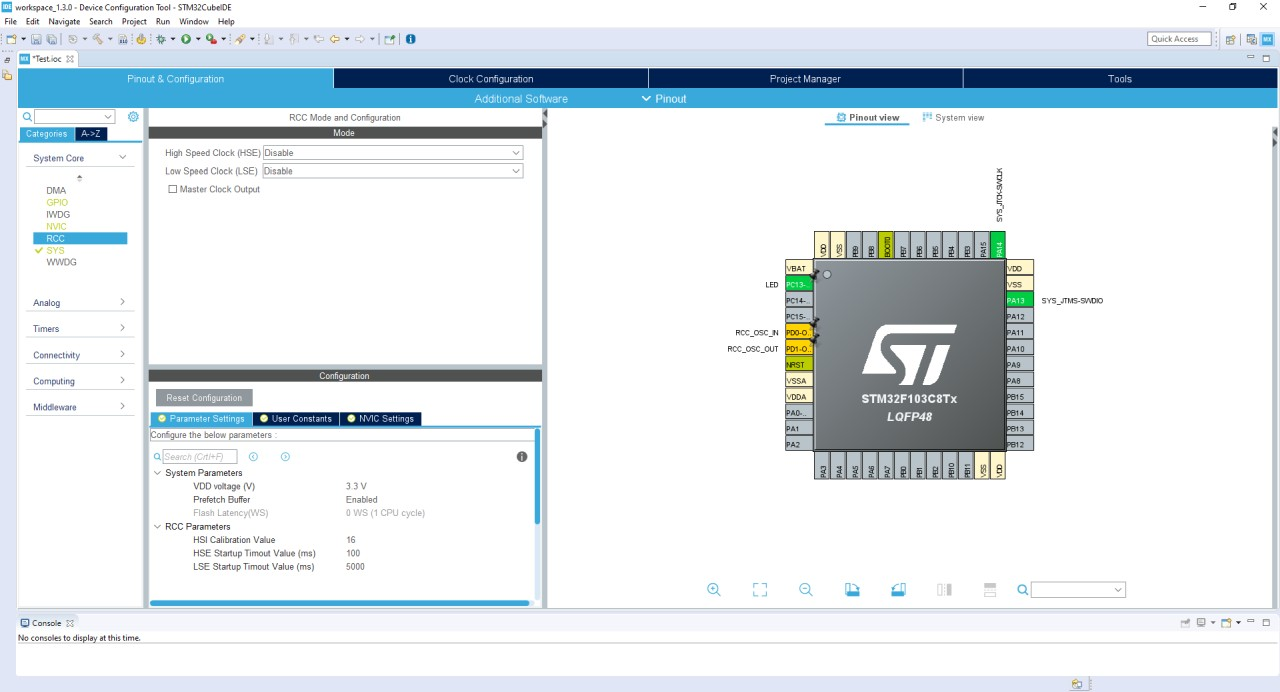
\includegraphics[width=0.9\textwidth]{../image/cube.jpg}
    \caption{Интерфейс STM32CubeIDE.}
	\end{figure}
	
	После выбора микроконтроллера STM32 создается проект и генерируется код инициализации. В любой момент разработки пользователь может вернуться к инициализации и настройке периферийных устройств и повторно создать код инициализации без какого-либо влияния на пользовательский код. Для разработки используется библиотека HAL. 
	
	Драйверы HAL включают в себя полный набор готовых к использованию функций, которые упрощают реализацию пользовательских приложений. Например, коммуникационные периферийные устройства содержат функции для инициализации и настройки периферийного устройства, управления передачей данных, обработки прерываний или DMA~\cite{hal}.
	
	Достоинства:
	\begin{itemize}
		\item поддержка различных ОС;
		\item расширенные возможности отладки;
		\item большое сообщество;
		\item автогенерация кода.
	\end{itemize}
	
	Недостатки:
	\begin{itemize}
		\item требовательность к ресурсам ПК;
		\item сложность настройки.
	\end{itemize}

\subsection{PlatformIO}

	PlatformIO --- удобная и расширяемая интегрированная среда разработки с набором профессиональных инструментов разработки, предоставляющая современные и мощные функции для ускорения и упрощения процесса разработки встраиваемых продуктов~\cite{plio}.
	
	\begin{figure}[h]
    \centering
    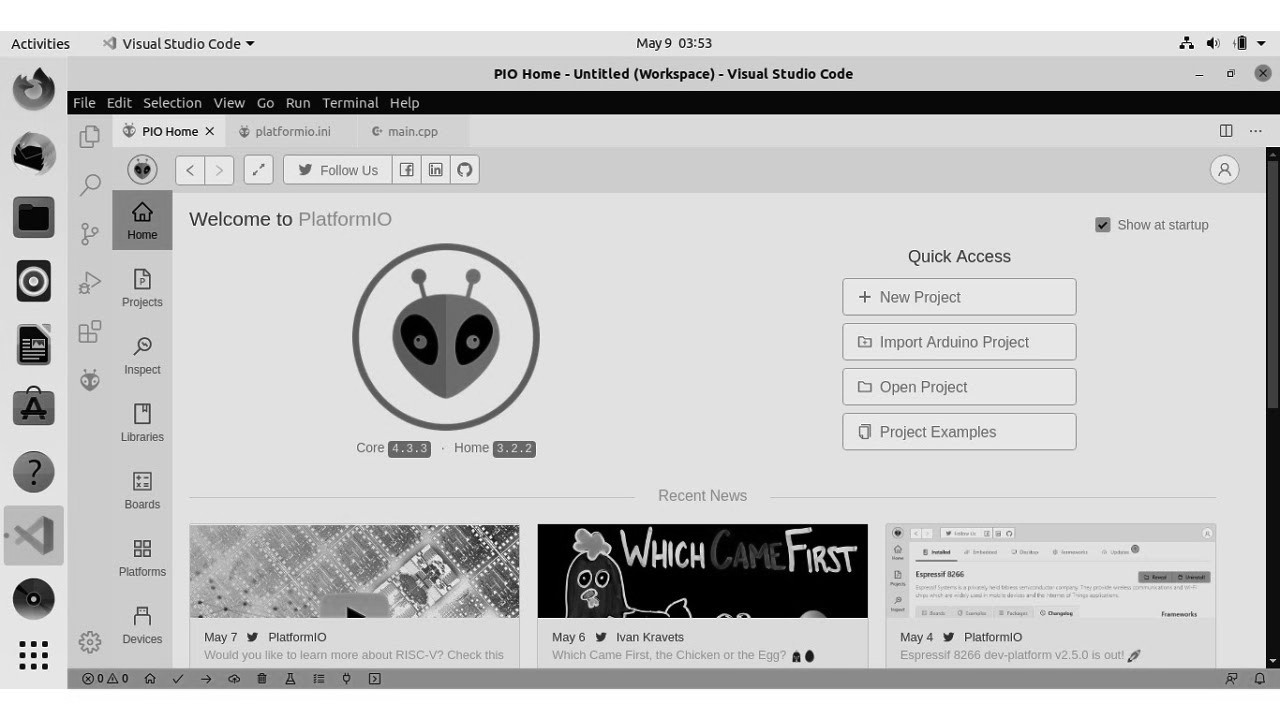
\includegraphics[width=0.9\textwidth]{../image/plio.jpg}
    \caption{Интерфейс PlatformIO.}
	\end{figure}
	
	Данная среда разработки является расширением для текстового редактора Visual Studio Code. VS Code --- это легкий, но мощный редактор кода, имеющий богатую экосистему расширений~\cite{docsplio}. Доступен для Windows, macOS и Linux. Работа в паре с VS Code позволяет удобно форматировать код и пользоваться расширениями для языков программирования.
	
	PlatformIO позволяет работать со многими микроконтроллерами и поддерживает множество фреймворков для них, а также библиотек. Ввиду такой широкой поддержки, для STM32 можно разрабатывать с удобной для себя библиотекой. Это может быть к примеру тот же HAL, что и в STM32CubeIDE или libopencm3. Проект libopencm3 (ранее известный как libopenstm32) направлен на создание бесплатной библиотеки микропрограмм с открытым исходным кодом (LGPL версии 3 или более поздней) для различных микроконтроллеров ARM Cortex-M3, включая ST STM32~\cite{lcm3}.


	Достоинства:
	\begin{itemize}
		\item поддержка различных ОС;
		\item быстрая компиляция;
		\item поддержка GitHub;
		\item возможность работать с разными фрэймворками и платформами.
	\end{itemize}
	
	Недостатки:
	\begin{itemize}
		\item высокий порог вхождения;
		\item сложность установки.
	\end{itemize}

	Попользовавшись обеими средами разработки и разными библиотеками, а также основываясь на достоинствах и недостатках была выбрана среда разработки PlatformIO в связке с библиотекой libopencm3.


\section{Алгоритм работы программы для генерации сигналов}

	Структурно устройство будет выглядеть следующим образом (рис. 2.8). Цифро-аналоговый преобразователь будет использоваться встроенный в микроконтроллер, а в качестве дисплея будет выступать OLED экран с разрешением 128 на 64 пикселя, работающий по интерфейсу I2C на контроллере SSD1306.
	
	\begin{figure}[H]
    \centering
    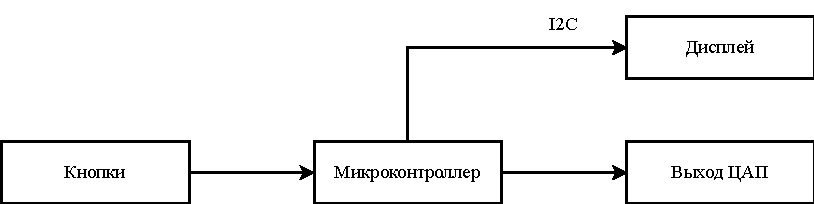
\includegraphics[width=1\textwidth]{../image/struct_gen.pdf}
    \caption{Структурная схема генератора сигналов.}
	\end{figure}
	
	Дисплей понадобится для вывода информации о форме сигнала, частоте и шаге регулировки частоты. Кнопки будут подключены напрямую к микроконтроллеру в количестве пяти штук для выполнения действий:
	\begin{enumerate}
		\item Уменьшить частоту;
		\item Увеличить частоту;
		\item Предыдущий сигнал;
		\item Следующий сигнал;
		\item Выбор шага.
	\end{enumerate}

	Программа должна выполнять три действия:
	
	\begin{enumerate}
		\item Вывод отсчёта в ЦАП (генерация сигнала);
		\item Обработка кнопок;
		\item Вывод информации на дисплей.
	\end{enumerate}
	
	
	Для цифро-аналогового преобразователя и кнопок выделим два таймера общего назначения. Таймер номер два будет использоваться для ЦАПа, а номер три для обработки кнопок. На примере третьего таймера рассмотрим его настройку. Алгоритм следующий:
	
	\begin{enumerate}
		\item Включить тактирование таймера;
		\item Задать стартовое значение;
		\item Установить предделитель;
		\item Установить период таймера;
		\item Включить прерывания от таймера;
		\item Запустить таймер.
	\end{enumerate}	 
	
	Кроме этого потребуется активировать прерывания и установить им приоритеты.
	
	Таймеры относятся к периферийным устройствам, а вся внутренняя периферия STM32 тактируется от шин APB1 и APB2 (Advanced Peripheral Bus)~\cite{tim}. В нашем случае таймеры тактируются от шины APB1, частота которой составляет 36 МГц~\cite{f103}. От предделителя зависит количество отсчётов таймера в секунду. Следовательно, если выставить предделитель 36000 получим следующее:
	
	\begin{center}
	$\dfrac{36*10^{6}}{36*10^{3}}=1000.$
	\end{center}
	
	Таймер будет делать 1000 отсчётов в секунду. Таким образом, 1 отсчёт таймера будет равняться 1 миллисекунде реального времени. Выставив период 250 получим прерывание от таймера каждые 250 мс. Данного времени хватит для обработки нажатия кнопки, тем самым решается проблема дребезга кнопок без использования программных или аппаратных задержек.
	
\begin{code}
\captionof{listing}{Настройка таймеров и прерываний}
\begin{minted}[mathescape,linenos,frame=lines,breaklines]{text}
static void timers_setup(void)
{
    rcc_periph_clock_enable(RCC_TIM2);
    rcc_periph_clock_enable(RCC_TIM3);

    /* Стартовое значение таймера */
    TIM_CNT(TIM2) = 0;
    TIM_CNT(TIM3) = 0;

    /* Предделитель 36MHz/36000 => 1000 отсчетов в секунду (счет начинается с 0, поэтому в предделителе и периоде нужно отнимать единичку) */
    TIM_PSC(TIM2) = 17;
    TIM_PSC(TIM3) = 35999;

    /* Период таймера */
    TIM_ARR(TIM2) = 9;
    TIM_ARR(TIM3) = 249;

    /* Включить прерывания */
    TIM_DIER(TIM2) |= TIM_DIER_UIE;
    TIM_DIER(TIM3) |= TIM_DIER_UIE;

    /* Запустить таймер */
    TIM_CR1(TIM2) |= TIM_CR1_CEN;
    TIM_CR1(TIM3) |= TIM_CR1_CEN;
}

static void nvic_setup(void)
{
    /* Активировать прерывания и установить приоритеты */
    nvic_enable_irq(NVIC_TIM2_IRQ);
    nvic_set_priority(NVIC_TIM2_IRQ, 2);

    nvic_enable_irq(NVIC_TIM3_IRQ);
    nvic_set_priority(NVIC_TIM3_IRQ, 1);
}
\end{minted}
\end{code}

	
	Таким образом, подпрограмма обработки кнопок будет размещена в обработчике прерывания от третьего таймера и будет состоять из функций для каждой кнопки.
	
	
\begin{code}
\captionof{listing}{Обработка кнопок}
\begin{minted}[mathescape,linenos,frame=lines,breaklines]{text}
void tim3_isr(void) // обработчик прерывания таймера3 (обработка кнопок)
{
    minus_freq();
    plus_freq();
    minus_signal(); // функции кнопок
    plus_signal();
    step_select();
    TIM_SR(TIM3) &= ~TIM_SR_UIF; // очистка флага прерывания
}
\end{minted}
\end{code}

	Обработка кнопок представлена следующей блок-схемой.	
	
	\begin{figure}[H]
    \centering
    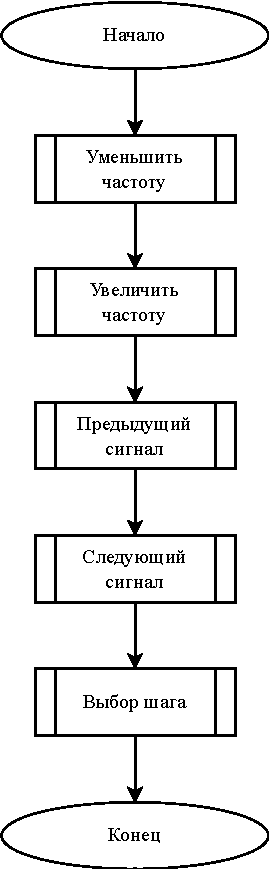
\includegraphics[width=0.3\textwidth]{../image/buttons.pdf}
    \caption{Блок-схема алгоритма функции кнопок.}
	\end{figure}
	
	Подпрограмма для вывода отсчёта в ЦАП будет размещена в обработчике прерывания второго таймера
	
\begin{code}
\captionof{listing}{Генерация сигнала}
\begin{minted}[mathescape,linenos,frame=lines,breaklines]{text}
void tim2_isr(void) // обработчик прерывания таймера2 (ЦАП)
{
    dac_load_data_buffer_single(signal[p_acc >> 8], RIGHT12, CHANNEL_2); // загрузка буфера в цап
    p_acc += p_step;             // шаг
    TIM_SR(TIM2) &= ~TIM_SR_UIF; // очистка флага прерывания
}
\end{minted}
\end{code}

	Работу подпрограммы генерации сигнала описывает следующая блок-схема.
	
	\begin{figure}[H]
    \centering
    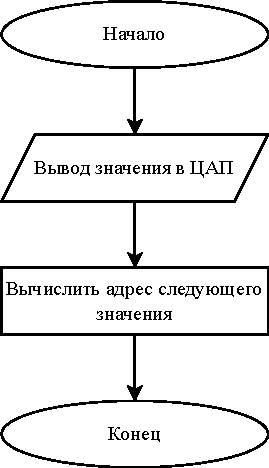
\includegraphics[width=0.325\textwidth]{../image/dac.pdf}
    \caption{Блок-схема алгоритма функции генерации сигнала.}
	\end{figure}

	Блок вычисления адреса содержит в себе выбранный метод прямого цифрового синтеза. Для аккумулятора фазы выделена переменная размером 2 байта. Старшая часть отвечает за адрес ячейки массива сигнала, состоящего из 256 отсчётов, а младшая за шаг в массиве. Размером же шага является код частоты, который прибавляется к аккумулятору фазы. Ввиду того, что размерность массива 256 точек и старшая часть аккумулятора больше 255 быть не может, то проблемы с выходом за границы массива не возникнет.
	
	Главный блок программы будет содержать в себе основные настройки периферии и вывод информации на дисплей. К периферии здесь относится настройка выводов микроконтроллера, таймеров, прерываний, ЦАП и интерфейса I2C для связи с дисплеем. 
	
	Интерфейс I2C широко применяется в микропроцессорных системах и его достоинство состоит в том, что передача данных идёт всего через две линии~\cite{schemat}. Одна линия для информации (SDA), вторая для синхросигнала (SCL). Для вывода информации на дисплей будет использоваться внешняя библиотека с функциями обновления, очистки и вывода строки~\cite{libdisp}. 
	
	В настройке выводов потребуется включить тактирование порта и выделить пять входов микроконтроллера для кнопок. Для цифро-аналогового преобразователя также потребуется включить тактирование, настроить выход и активировать его работу. Настройка I2C будет проходить по следующему алгоритму:
	
	\begin{enumerate}
	\item Включение тактирования;
	\item Настройка альтернативных функций SCL и SDA;
	\item Отключение I2C перед изменением конфигурации;
	\item Сброс состояния;
	\item Установка стандартного режима работы;
	\item Установка частоты периферии;
	\item Настройка тактовой частоты шины;
	\item Задать время нарастания сигналов;
	\item Включить подтверждение при получении данных;
	\item Запуск интерфейса I2C.
	\end{enumerate}
	
	Стандартный режим работы I2C --- стандартная тактовая частота работы 100 кГц. Тактируется интерфейс также от шины APB1 --- 36 МГц. По спецификации микроконтроллера устанавливается частота шины~\cite{f103}.
	
	\begin{figure}[H]
    \centering
    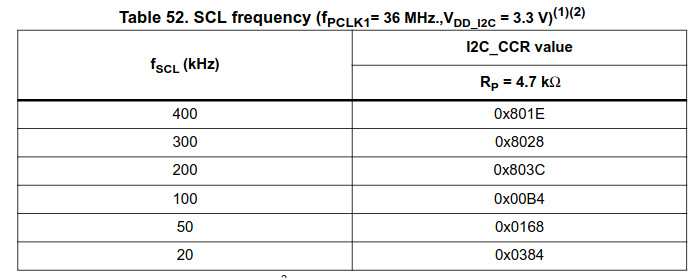
\includegraphics[width=0.75\textwidth]{../image/i2c_ccr.png}
    \caption{Частота шины.}
	\end{figure}
	
	Так как частота тактирования 36 МГц, то время цила будет $\dfrac{1}{36}=28$ нс. В характеристиках I2C указано время нарастания сигналов $t_{r}=300$ нс~\cite{f103}.
	
	\begin{figure}[H]
    \centering
    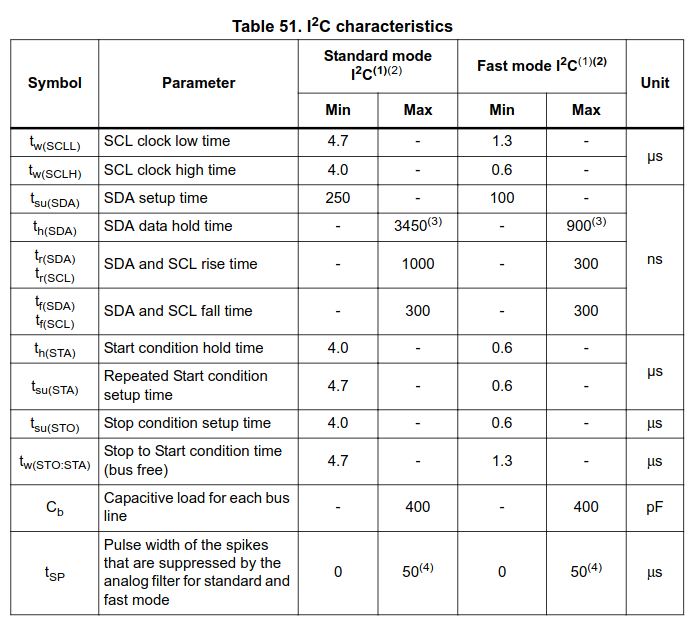
\includegraphics[width=0.75\textwidth]{../image/i2c_rise.png}
    \caption{Характеристики I2C.}
	\end{figure}
	
	По формуле рассчитаем нужное значение для установки времени нарастания~\cite{czssd1306}.
	\begin{center}
	$I2C\_TRISE=\dfrac{t_{r}}{TPCL1}+1=\dfrac{300}{28}+1=37$.
	\end{center}

\begin{code}
\captionof{listing}{Функции настроек выводов, ЦАП и I2C}
\begin{minted}[mathescape,linenos,frame=lines,breaklines]{text}
static void gpio_setup(void)
{
    // rcc_periph_clock_enable(RCC_GPIOD); // тактирование портов
    rcc_periph_clock_enable(RCC_GPIOB);
    gpio_set_mode(GPIOB, GPIO_MODE_INPUT, GPIO_CNF_INPUT_PULL_UPDOWN, GPIO9 | GPIO5 | GPIO6 | GPIO7 | GPIO8); // входы для кнопок, подтянуты к земле
    // gpio_set_mode(GPIOD, GPIO_MODE_OUTPUT_50_MHZ, GPIO_CNF_OUTPUT_PUSHPULL, GPIO2);
}

static void dac_setup(void)
{
    rcc_periph_clock_enable(RCC_GPIOA);
    gpio_set_mode(GPIOA, GPIO_MODE_OUTPUT_2_MHZ, GPIO_CNF_OUTPUT_ALTFN_PUSHPULL, GPIO5);
    rcc_periph_clock_enable(RCC_DAC); // тактирование цапа и настройка вывода
    dac_enable(CHANNEL_2);            // включить цап
}

static void i2c_setup(void){
    // Включение тактирования периферийного оборудования для I2C2
    rcc_periph_clock_enable(RCC_I2C2);
    
    /*
     * Настройка альтернативных функций для пинов SCL и SDA интерфейса I2C2.
     * Это необходимо для подключения I2C устройств к микроконтроллеру через эти
 пины.
     */
    gpio_set_mode(GPIOB, GPIO_MODE_OUTPUT_50_MHZ,
                  GPIO_CNF_OUTPUT_ALTFN_OPENDRAIN,
                  GPIO_I2C2_SCL | GPIO_I2C2_SDA);
    
    // Отключение I2C перед изменением конфигурации
    i2c_peripheral_disable(I2C2);
    
    // Сброс состояния периферийного устройства I2C2
    i2c_reset(I2C2);
    
    // Установка стандартного режима работы I2C 
    i2c_set_standard_mode(I2C2);
    
    // Установка частоты периферии
    i2c_set_clock_frequency(I2C2, I2C_CR2_FREQ_36MHZ);
    
    // Настройка тактовой частоты шины; 
    i2c_set_ccr(I2C2, 0xB4);
    
    // Установка времени подъема сигнала SDA после завершения операции чтения/записи
    i2c_set_trise(I2C2, 0x25);
    
    // Включение подтверждения при получении данных от устройства
    i2c_enable_ack(I2C2);
    
    // Включение периферийного устройства I2C2
    i2c_peripheral_enable(I2C2);
}
\end{minted}
\end{code}
	
	
	На рис. 2.10 представлена блок-схема алгоритма главной функции.
	
	\begin{figure}[H]
    \centering
    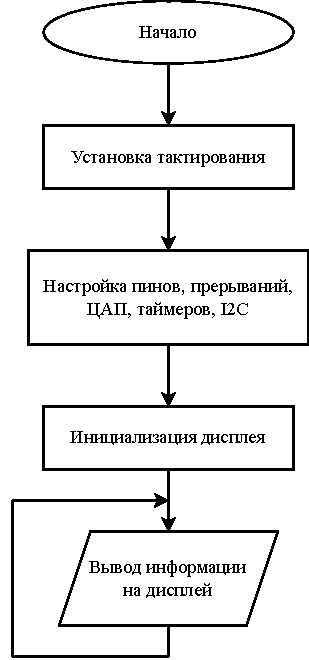
\includegraphics[width=0.375\textwidth]{../image/main.pdf}
    \caption{Блок-схема алгоритма главной функции.}
	\end{figure}
	
\begin{code}
\captionof{listing}{Главная функция программы}
\begin{minted}[mathescape,linenos,frame=lines,breaklines]{text}
int main(void)
{
    rcc_clock_setup_in_hse_8mhz_out_72mhz(); // установка тактирования
    gpio_setup();
    nvic_setup();
    dac_setup();
    timers_setup();
    i2c_setup();
    ssd1306_init(I2C2, DEFAULT_7bit_OLED_SLAVE_ADDRESS, 128, 64); // инициализация дисплея

    int f = 0;       // переменная частоты
    wchar_t freq[8]; // буфер для wchar_t строки
    while (1)
    {
        f = p_step / 24 * 125;
        swprintf(freq, sizeof(freq) / sizeof(wchar_t), L"%d", f); // Использование swprintf для преобразования int в wchar_t*
        /*  вывод информации на дисплей  */
        ssd1306_clear();
        ssd1306_drawWCharStr(0, 0, white, nowrap, L"Форма сигнала:");
        switch (num_sig)
        {
        case 1:
            ssd1306_drawWCharStr(0, 8, white, nowrap, L"Синус");
            break;
       	...
        case 5:
            ssd1306_drawWCharStr(0, 8, white, nowrap, L"Пила Правая");
            break;
        }
        ssd1306_drawWCharStr(0, 16, white, nowrap, L"Частота(Гц)");
        ssd1306_drawWCharStr(64, 16, white, nowrap, freq);
        ssd1306_drawWCharStr(0, 32, white, nowrap, L"Шаг(Гц)");
        switch (num_step)
        {
        case 1:
            ssd1306_drawWCharStr(64, 32, white, nowrap, L"125");
            break;
        ...
        case 4:
            ssd1306_drawWCharStr(64, 32, white, nowrap, L"1000");
            break;
        }
        ssd1306_refresh();
    }

    return 0;
}
\end{minted}
\end{code}
	
	Полный код программы содержится в приложении. После написания программы произведём сборку проекта и получим сообщение об успешной компиляции (рис. 2.12).
	
	\begin{figure}[H]
    \centering
    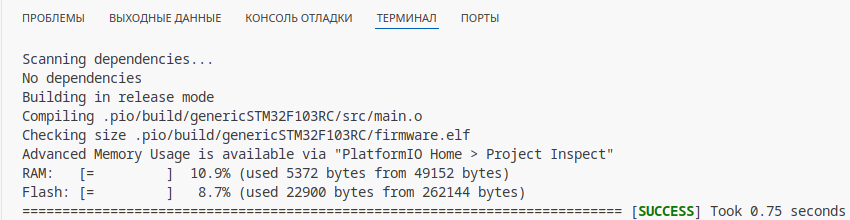
\includegraphics[width=1\textwidth]{../image/compile.png}
    \caption{Компиляция проекта.}
	\end{figure}
	
	Для более подробной информации проверим проект с помощью функции <<Inspect>>.
	
	\begin{figure}[H]
    \centering
    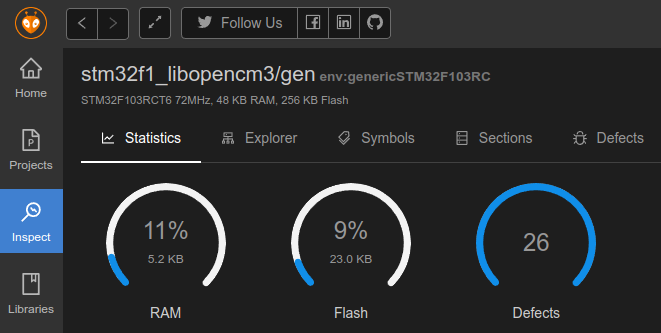
\includegraphics[width=0.8\textwidth]{../image/inspect.png}
    \caption{Проверка проекта.}
	\end{figure}
	
	Среда разработки описала занимаемую память и нашла дефекты в проекте.
	
	\begin{figure}[H]
    \centering
    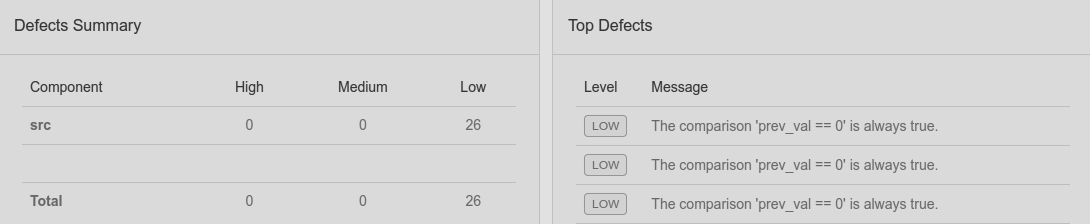
\includegraphics[width=1\textwidth]{../image/defects.png}
    \caption{Дефекты проекта.}
	\end{figure}
	
	Дефекты оказались незначительные и на работу программы влияния не оказывают.
	
\section{Вывод по второй главе}
	
	Таким образом, для реализации генератора сигналов был выбран микроконтроллер STM32F103RCT6 с использованием среды разработки PlatformIO и библиотеки libopencm3. Определен четкий план действий, включающий структуру программы, алгоритмы работы с цифро-аналоговым преобразователем, кнопками и дисплеем. Была разработана и скомпилирована результирующая программа, которая будет протестирована на макете устройства.

	
	

\chapter{ПРОЕКТИРОВАНИЕ И ТЕСТИРОВАНИЕ ГЕНЕРАТОРА СИГНАЛОВ}
\section{Проектирование генератора сигналов}
	По структурной схеме (рис. 2.7) создадим фрагмент схемы электрической принципиальной. 
	
	\begin{figure}[H]
    \centering
    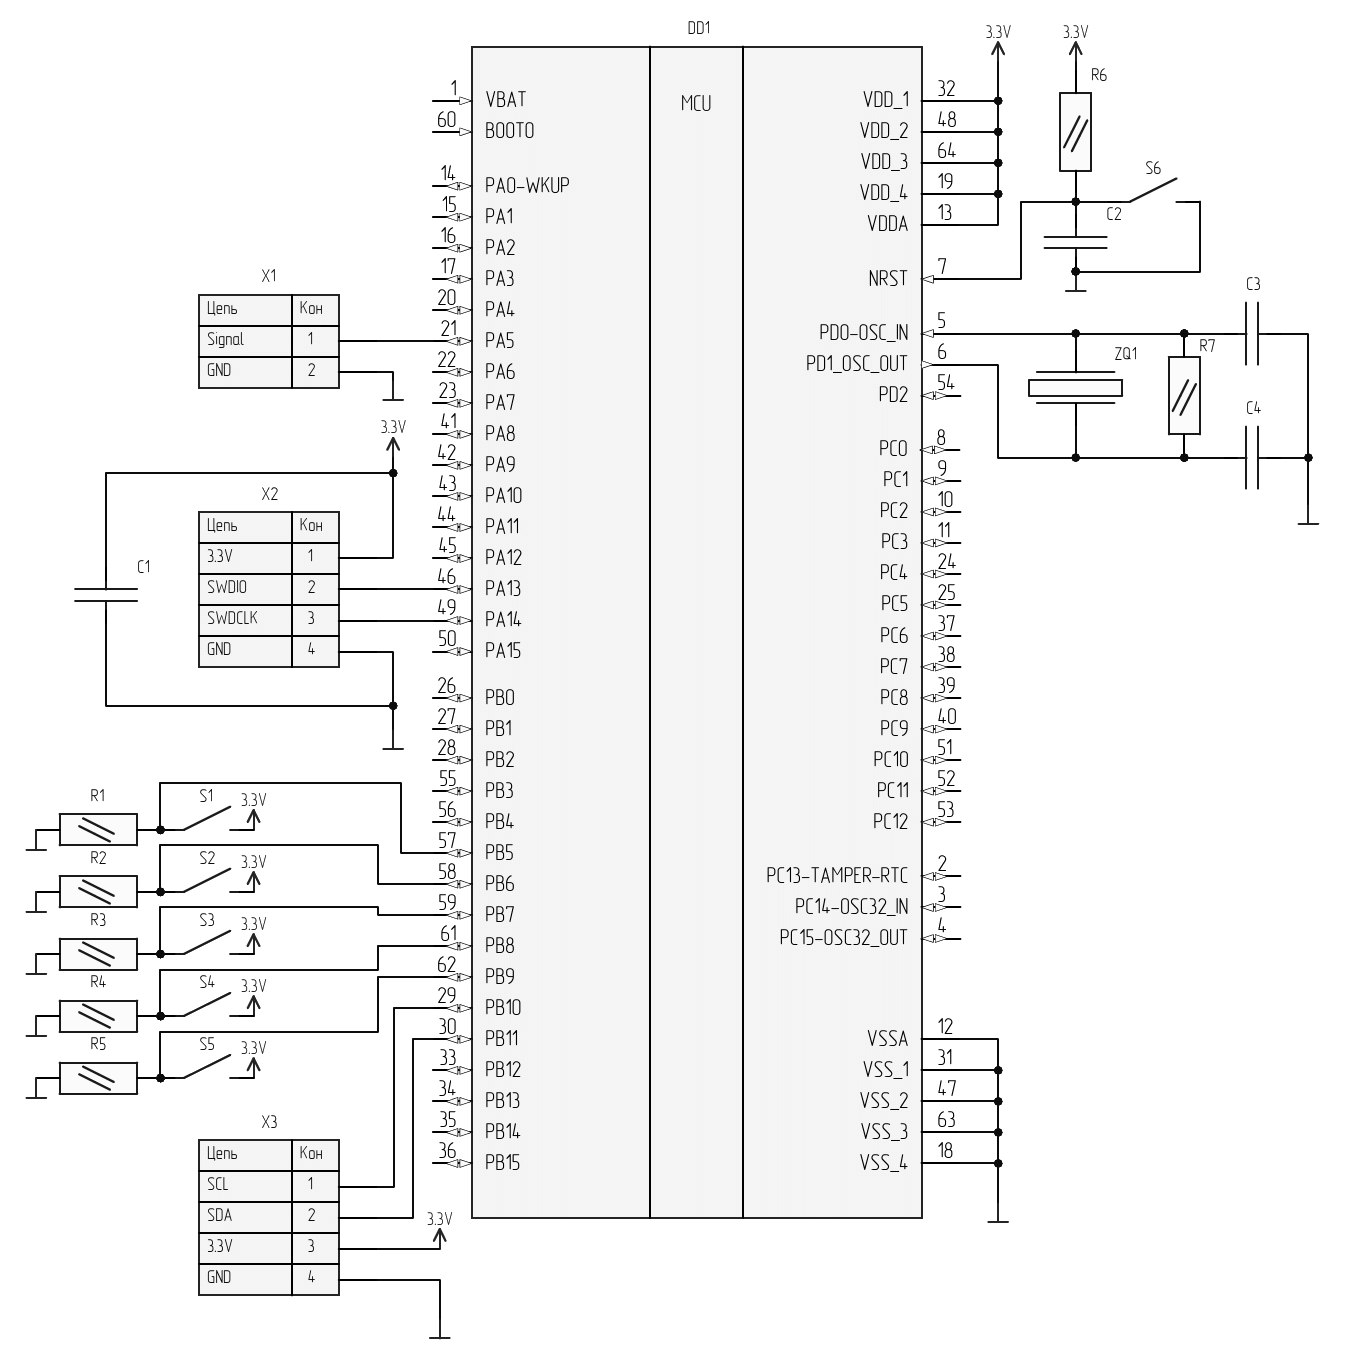
\includegraphics[width=1\textwidth]{../image/scheme-cropped.png}
    \caption{Фрагмент схемы электрической принципиальной.}
	\end{figure}
	
	Просто так контроллер работать не сможет. Необходим внешний кварцевый резонатор для стабилизации частоты системного тактового генератора, а также функция сброса. Эти узлы уже реализованы на отладочной плате микроконтроллера. Питание схемы будет подаваться через разъём SWD.
		
	Для улучшения генерации будет задействован встроенный в цифро-аналоговый преобразователь выходной буфер. При его использовании он будет срезать сигнал сверху и снизу на 0.2В, поэтому значения тоже следует срезать на эту же величину для корректной генерации.
	
	В документе от STM про работу с цифро-аналоговым преобразователем есть формула для расчета выходного напряжения~\cite{an3126}.
	
	\begin{gather}
	DAC_{output} = V_{REF}*\dfrac{DOR}{DAC_{MaxDigitalValue} + 1},
	\end{gather}
	
	где $DAC_{output}$ --- выходное напряжение ЦАП,
	
	$V_{REF}$ --- опорное напряжение,
	
	$DOR$ --- цифровое значение выходного напряжения,
	
	$DAC_{MaxDigitalValue}$ --- максимальное значение $DOR$.
	
	Нам нужно найти какое значение соответствует напряжению 0.2В. Выразим DOR и подставим имеющиеся значения.
	
	\begin{center}
	$DOR = \dfrac{V_{REF}}{DAC_{output}}*DAC_{MaxDigitalValue} + 1 = \dfrac{3.3}{0.2}*(4095+1) = 248.$
	\end{center}
	
	Поэтому для отсчётов нужно будет указать смещение от нуля 248, а максимальное значение 4095 меньше на 248, то есть 3847. 
	
	Для управления установлены 5 кнопок, для которых выделены выводы PB5 - PB9. Постоянно быть подключенными к напряжению или земле выводы не могут, т. к. не будет возможности подавать на них какой-либо информационный сигнал. На выводы могут наводиться произвольные потенциалы, что негативно влияет на работу схемы. Подобные потенциалы имитируют сигналы, которые не предусмотрены. Из-за них может нарушиться логика работы, поэтому их принято фиксировать~\cite{schemat}. 
	
	Для этого используют подтягивающие (Pull - up) или заземляющие (Pull - down) резисторы. Они создают цепь, которая обеспечивает подтяжку сигнала к напряжению питания или земле. Если резисторы имеют большие сопротивления, то сигналы относят к слабым. При подключении сильных информационных сигналов происходит преодоление слабых и функциональность схемы не нарушается~\cite{butres}.
	
	\begin{figure}[H]
    \centering
    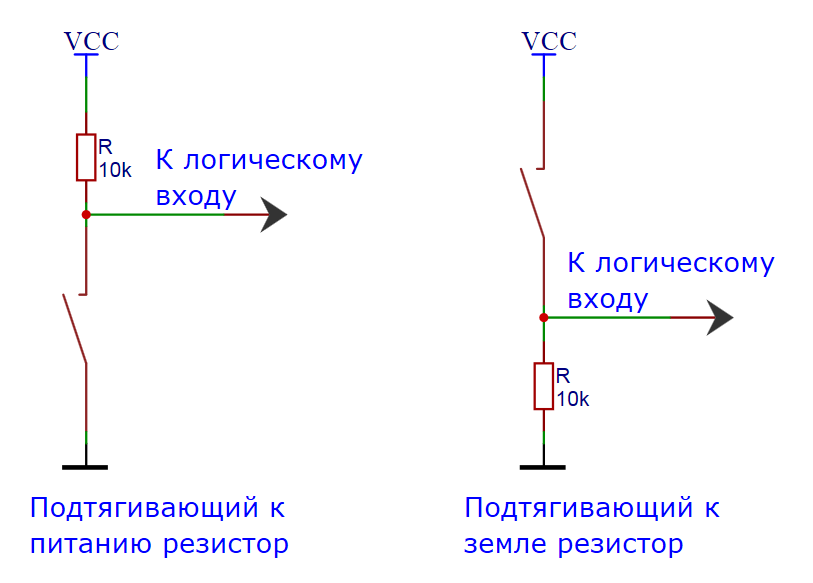
\includegraphics[width=0.55\textwidth]{../image/res.png}
    \caption{Pull-up и Pull - down резисторы.}
	\end{figure}
	
	В схеме устройства будет использоваться подтяжка к земле для считывания высокого уровня сигнала, то есть будет использоваться прямая логика. Рассчитаем минимальное и максимальное сопротивление заземляющего резистора.
	\begin{gather}
	R_{min} = \dfrac{V_{0}}{I_{max}},
	\end{gather}
	
	где $V_{0}$ --- напряжение логического нуля,
	
	$I_{max}$ --- максимальный ток вывода.
	
	Согласно спецификации микроконтроллера напряжение логического нуля составляет 1,16 В, а максимальный протекающий ток через пин может быть 25 мА~\cite{f103}. 
	
\begin{center}
	$R_{min} = \dfrac{1,16}{25*10^{-3}} = 46,4$ Ом.
\end{center}

	Для расчета максимального сопротивления формула следующая:
	\begin{gather}
	R_{max} = \dfrac{t}{C_{I/O}},
	\end{gather}
	
	где $t$ --- время нарастания сигнала,
	
	$C_{I/O}$ --- ёмкость вывода.
	
	Ёмкость вывода составляет 5 пФ, время нарастания возьмём 1 микросекунду (стандартный сигнал 100 кГц).
	
\begin{center}
	$R_{max} = \dfrac{1*10^{-6}}{5*10^{-12}} = 200$ кОм.
\end{center}	

	Из расчётов можно сделать вывод, что номинал резистора расположен в следующих границах.
	
\begin{center}
	$46,4$ Ом$ < R < 200$ кОм.
\end{center}	

	Разброс довольно большой, но из практики известно, что подтягивающий резистор имеет номинал 1 - 10 кОм.
	
	Для линий I2C также используются подтягивающие резисторы, которые уже установлены на дисплее.
	
	\begin{figure}[H]
    \centering
    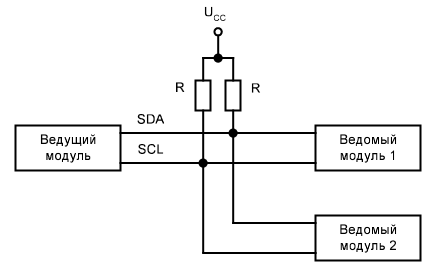
\includegraphics[width=0.525\textwidth]{../image/i2c.png}
    \caption{Организация интерфейса.}
	\end{figure}
	
	Интерфейс в микроконтроллере расположен на выводах PB10 (SCL) и PB11 (SDA). Также для дисплея потребуется питание 3.3 В.
	
	Дисплей и кнопки расположим на макетной плате размером 50 на 50 мм.
	
	\begin{figure}[H]
    \centering
    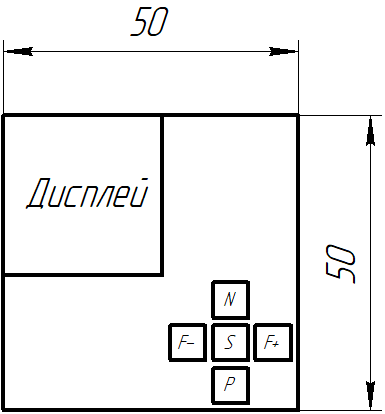
\includegraphics[width=0.45\textwidth]{../image/func_gen.png}
    \caption{Схема расположения периферии.}
	\end{figure}
	
	Назначения кнопок:
	\begin{enumerate}
	\item F- --- уменьшить частоту;
	\item F+ --- увеличить частоту;
	\item P --- предыдущий сигнал;
	\item N --- следующий сигнал;
	\item S --- переключить шаг по частоте.
	\end{enumerate}
	
	В результате сборки получилась плата с периферией.

	\begin{figure}[H]
    \centering
    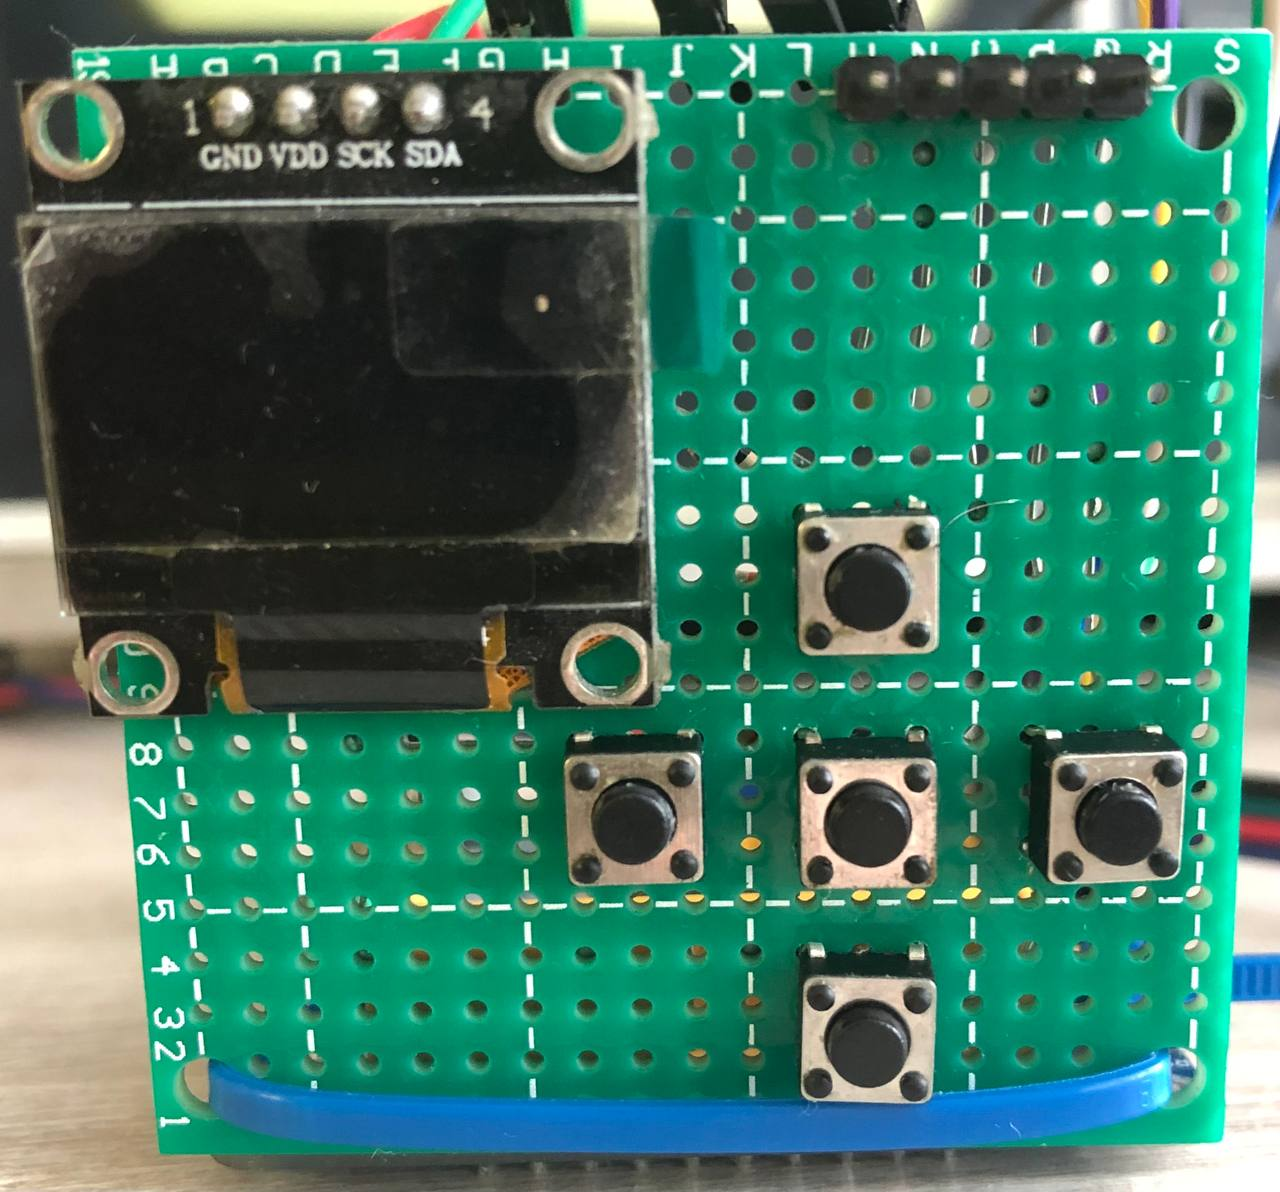
\includegraphics[width=0.5\textwidth]{../image/m1.jpeg}
    \caption{Плата периферии.}
	\end{figure}	
	
	Макет устройства будет состоять из отладочной платы микроконтроллера и полученной платы периферии. Обе части будут соединены проводами. Выход цифро-аналогового преобразователя, на котором генерируется сигнал, расположен на отладочной плате. В результате конструирования получился следующий макет устройства (рис. 3.6).

	\begin{figure}[H]
    \centering
    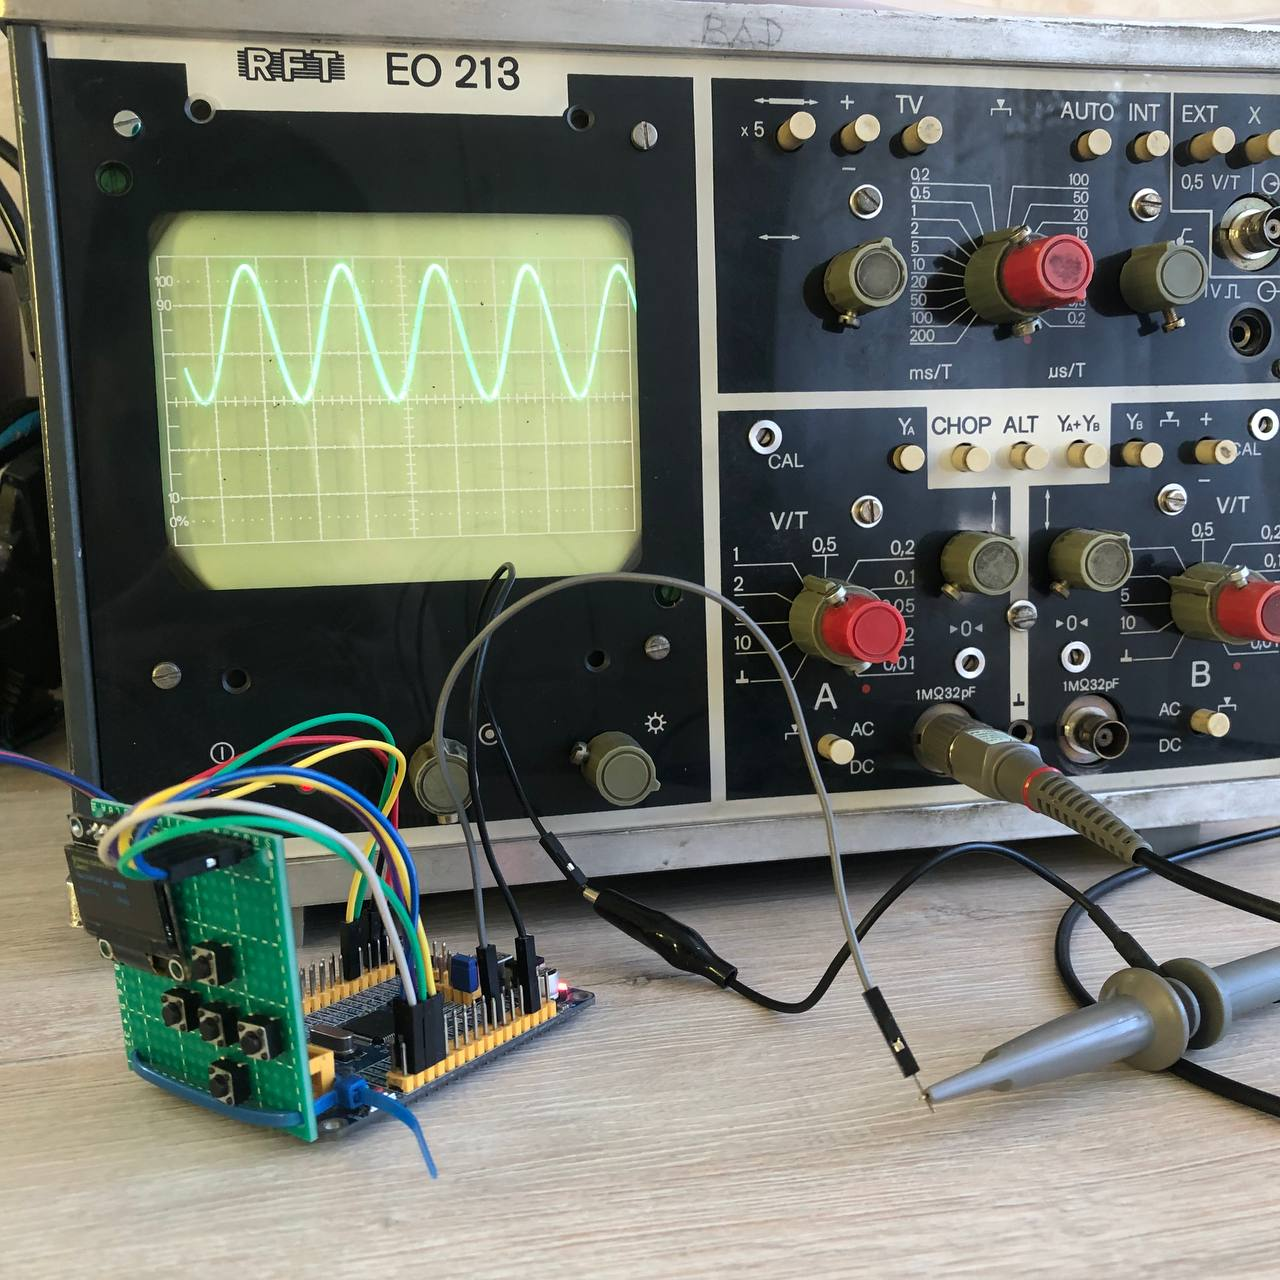
\includegraphics[width=0.5\textwidth]{../image/m2.jpg}
    \caption{Макет устройства.}
	\end{figure}	

\section{Тестирование генератора сигналов}
	
	Протестируем работоспособность полученного устройства. Будем отслеживать состояние устройства и информацию в отладчике. В отладчике будем отслеживать следующие переменные:
	\begin{itemize}
	\item f --- расчетная частота;
	\item step --- код частоты (шаг по частоте);
	\item num\_step --- номер шага;
	\item num\_sig --- номер сигнала;
	\item signal --- буфер сигнала.
	\end{itemize}		
	
	После запуска устройства на экране появляются строки с пустыми параметрами формы сигнала, частоты и шага (рис. 3.7). 

	\begin{figure}[H]\captionsetup[subfigure]{font=normalsize}
     \begin{subfigure}[H]{0.5\textwidth}
         \centering
         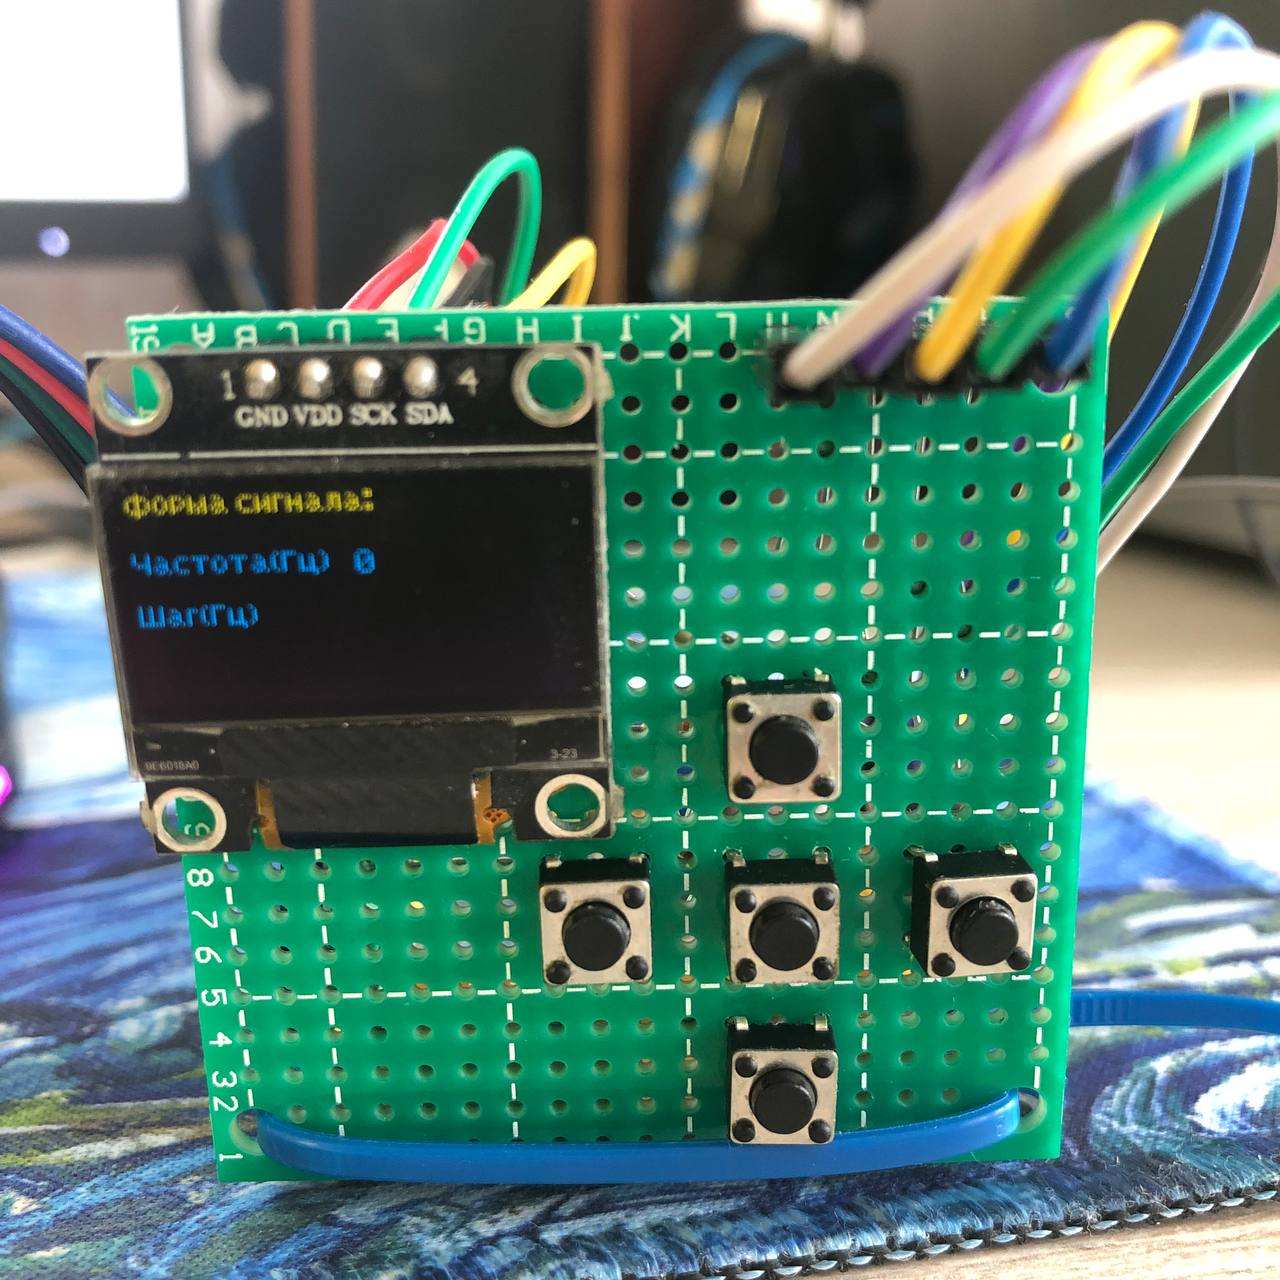
\includegraphics[width=0.6\textwidth]{../image/test0_u_s.jpg}
         \caption{Состояние устройства.}
     \end{subfigure}
     \hfill
     \begin{subfigure}[H]{0.5\textwidth}
         \centering
         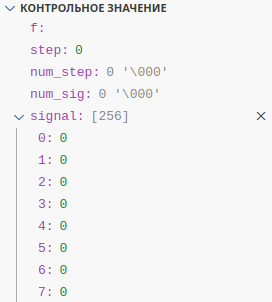
\includegraphics[width=0.525\textwidth]{../image/test0_o_s.png}
         \caption{Состояние в отладчике.}
     \end{subfigure}
        \caption{Начальное состояние устройства при запуске.}
	\end{figure}
	
	Логика работы дисплея описана блок-схемой (рис. 3.8).
	
	\begin{figure}[H]
    \centering
    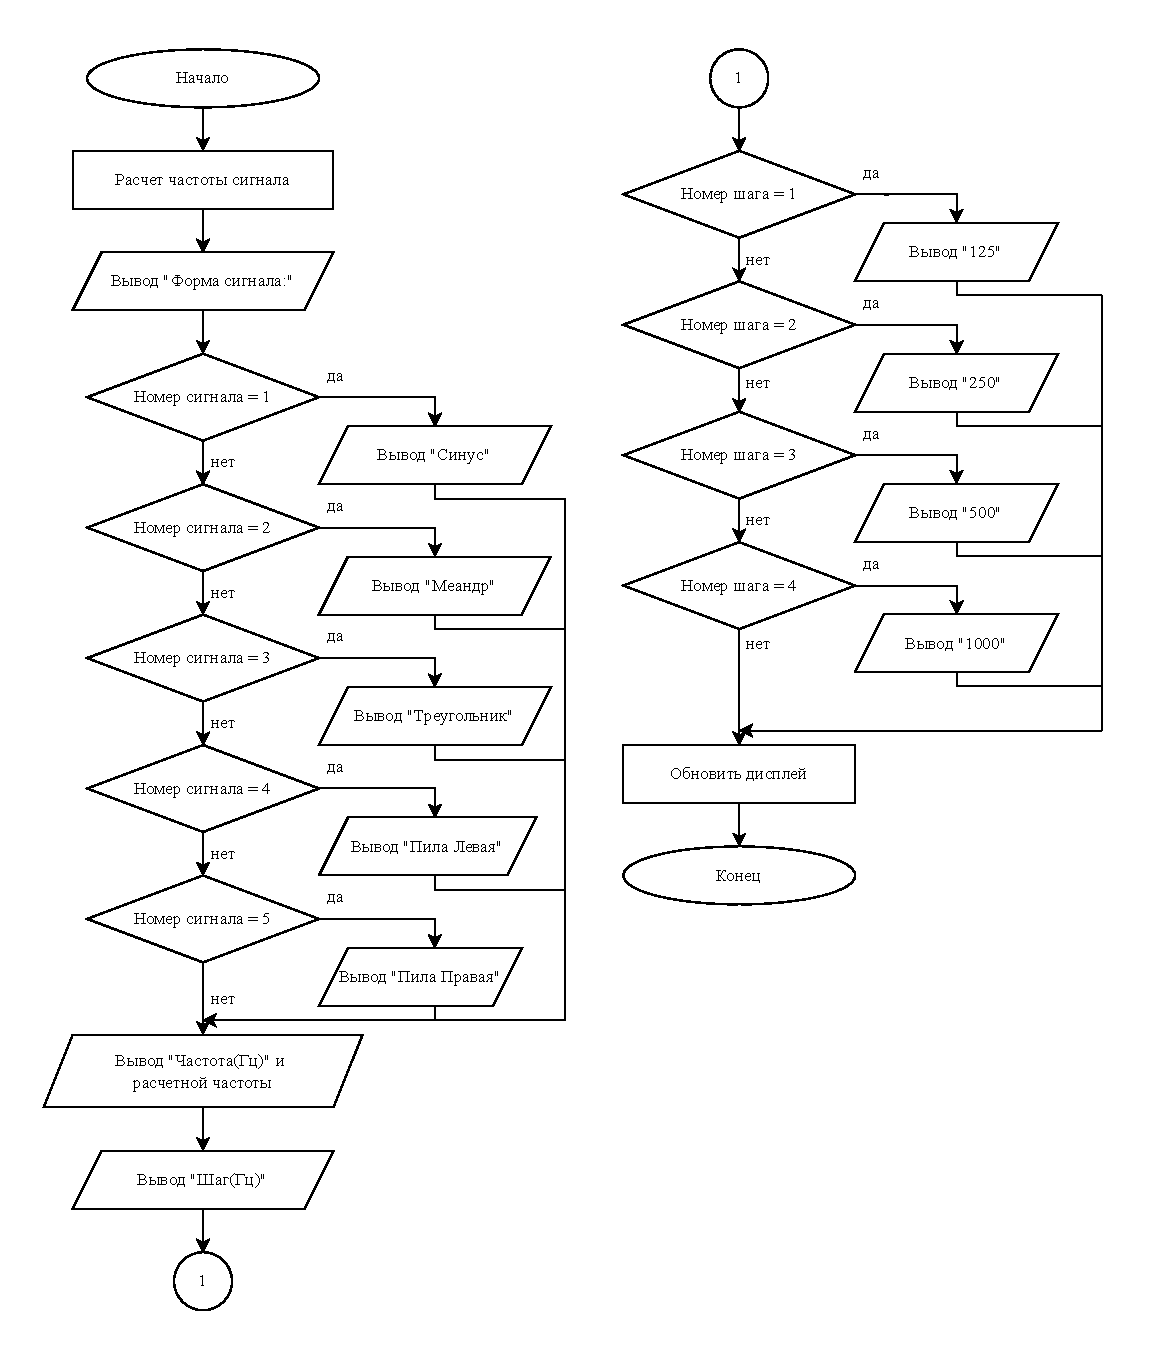
\includegraphics[width=0.775\textwidth]{../image/display.pdf}
    \caption{Блок-схема алгоритма работы дисплея.}
	\end{figure}	
	
	Требуется выставить параметры сигнала. Клавишами N и P выбирается форма сигнала. При нажатии клавиши N выполняется алгоритм, описанный блок-схемой (рис. 3.10). Для клавиши P алгоритм отличается только тем, что номер сигнала нужно декрементировать.
	
	\begin{figure}[H]
    \centering
    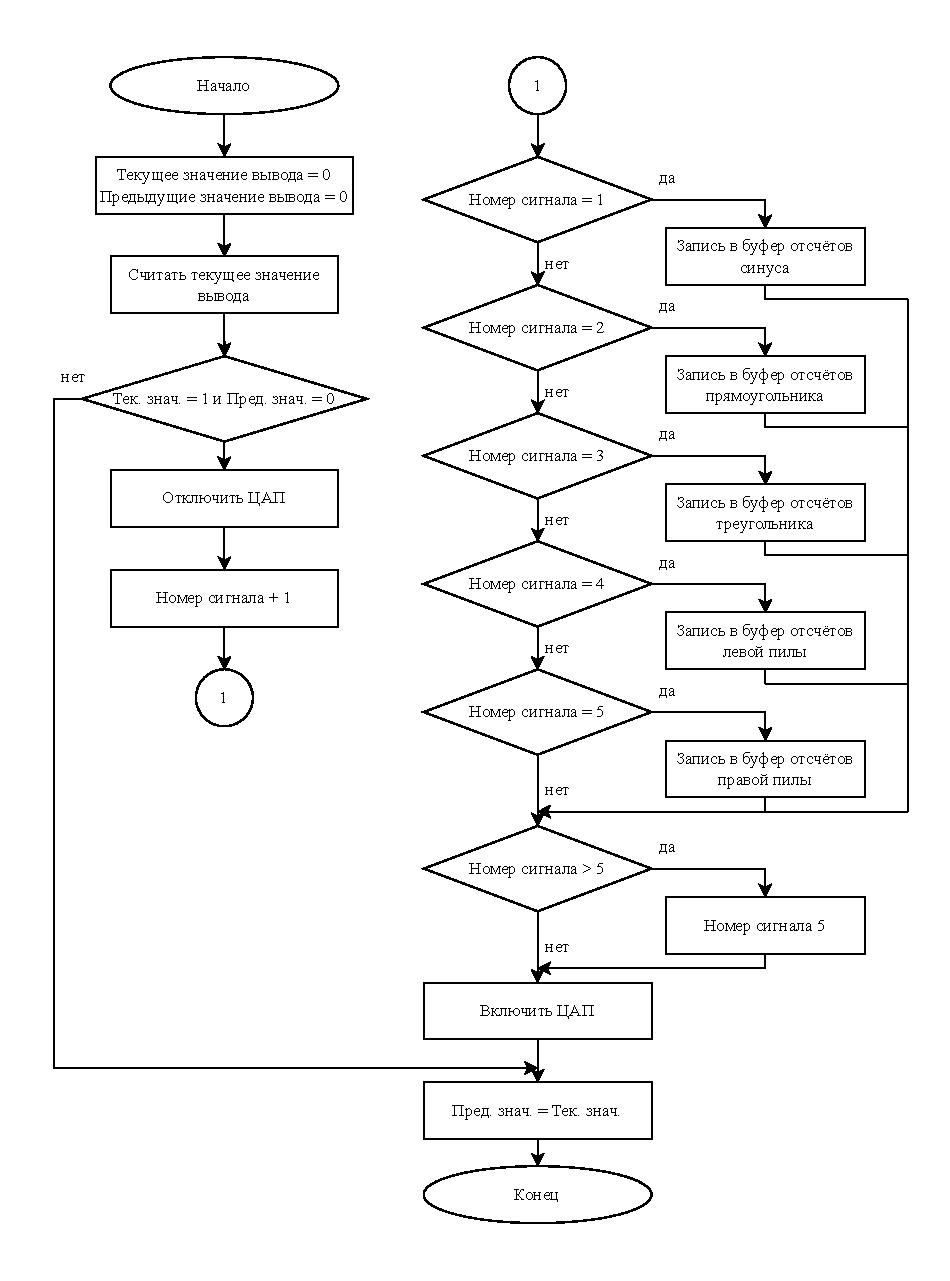
\includegraphics[width=0.8\textwidth]{../image/plus_signal.pdf}
    \caption{Блок-схема алгоритма выбора следующего сигнала.}
	\end{figure}	
	
	При выборе сигнала пользователь листает формы сигнала, а микроконтроллер заполняет буфер отсчётами выбранного сигнала. Выберем сигнал синуса.
	\begin{figure}[H]\captionsetup[subfigure]{font=normalsize}
     \begin{subfigure}[H]{0.5\textwidth}
         \centering
         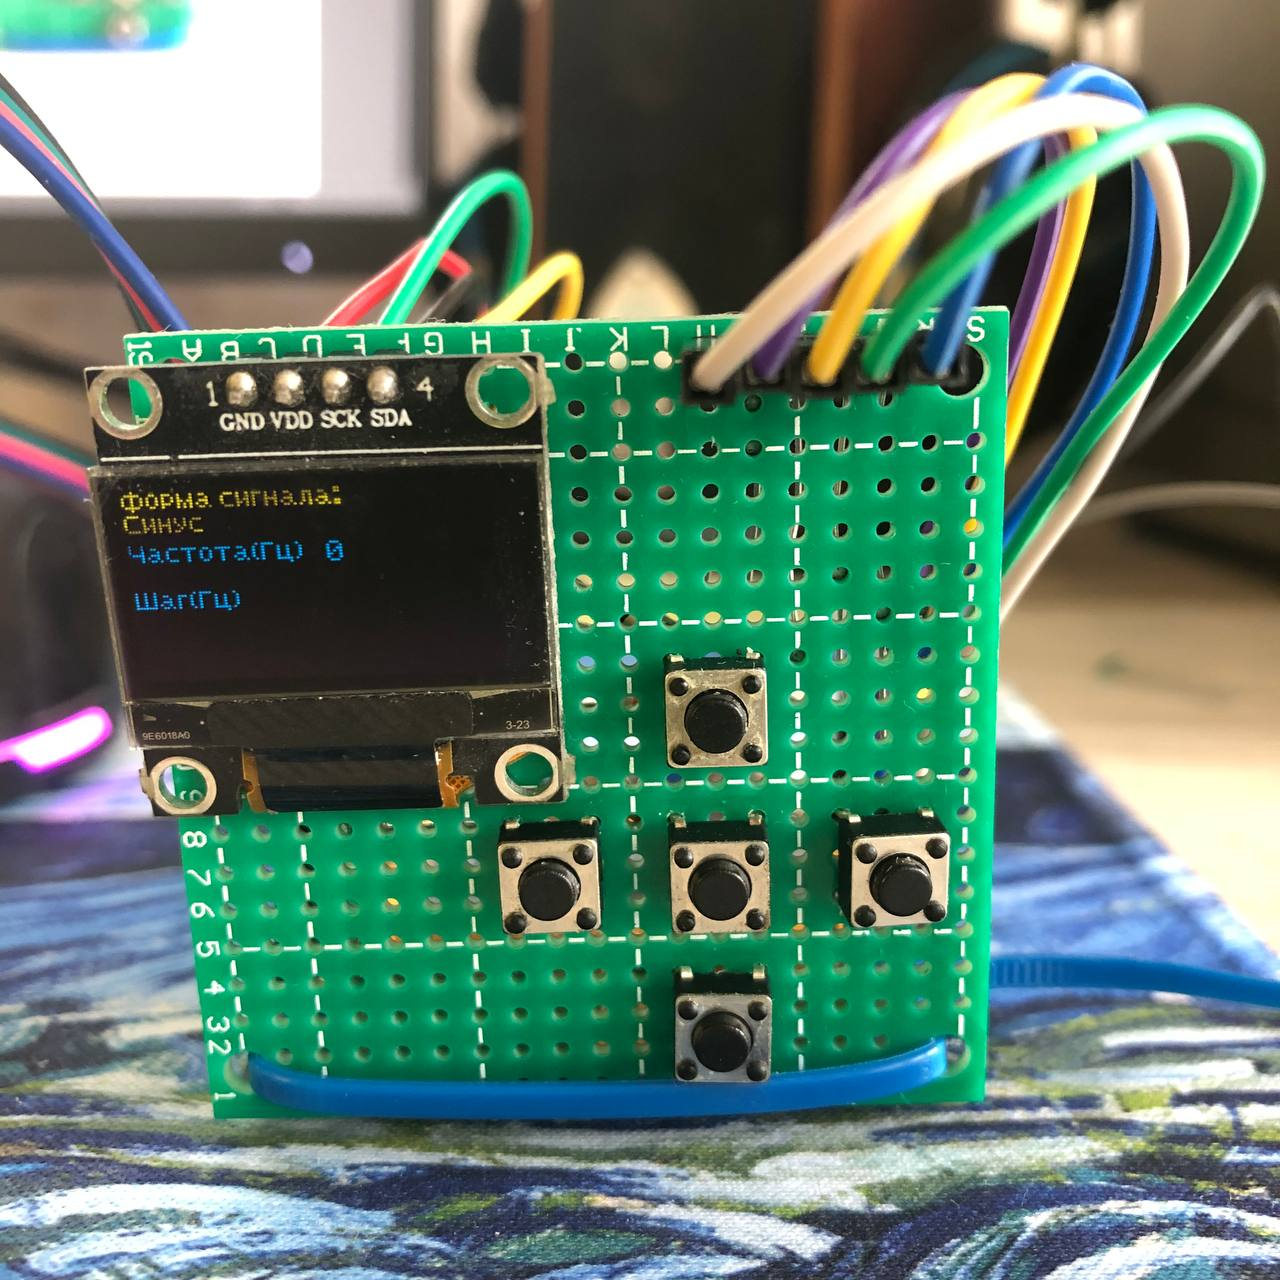
\includegraphics[width=0.6\textwidth]{../image/test1_u_s.jpg}
         \caption{Состояние устройства.}
     \end{subfigure}
     \hfill
     \begin{subfigure}[H]{0.5\textwidth}
         \centering
         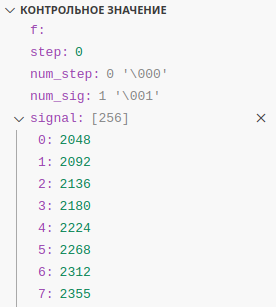
\includegraphics[width=0.525\textwidth]{../image/test1_o_s.png}
         \caption{Состояние в отладчике.}
     \end{subfigure}
        \caption{Процедура выбора синусоидального сигнала.}
	\end{figure}

	Теперь нужно выбрать величину шага, с которым будет регулироваться частота сигнала. Алгоритм для установки шага следующий (рис. 3.16).
	
	\begin{figure}[H]
    \centering
    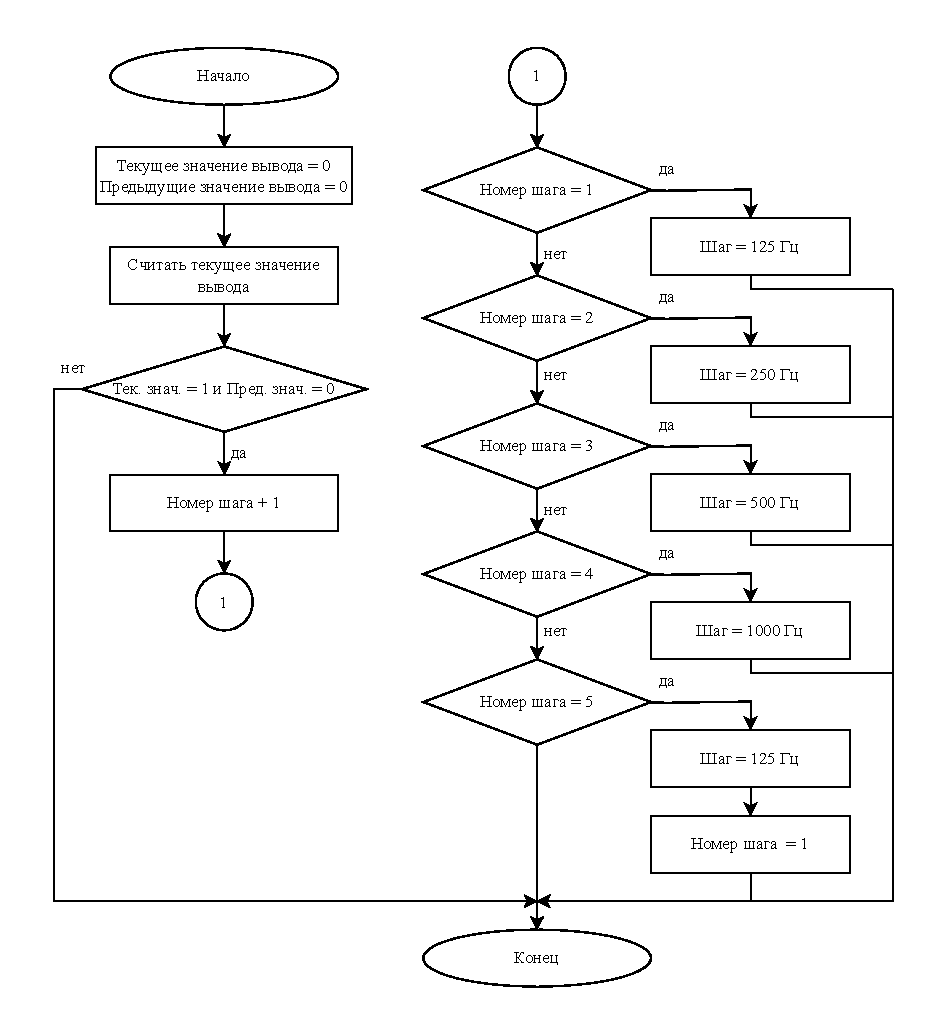
\includegraphics[width=0.8\textwidth]{../image/step_select.pdf}
    \caption{Блок-схема алгоритма выбора шага.}
	\end{figure}	
	
	Как можно заметить из блок-схемы всего есть 4 шага:
	\begin{enumerate}
		\item 125 Гц;
		\item 250 Гц;
		\item 500 Гц;
		\item 1000 Гц.
	\end{enumerate}
	
	Выберем для примера шаг 125 Гц.
	
	\begin{figure}[H]\captionsetup[subfigure]{font=normalsize}
     \begin{subfigure}[H]{0.5\textwidth}
         \centering
         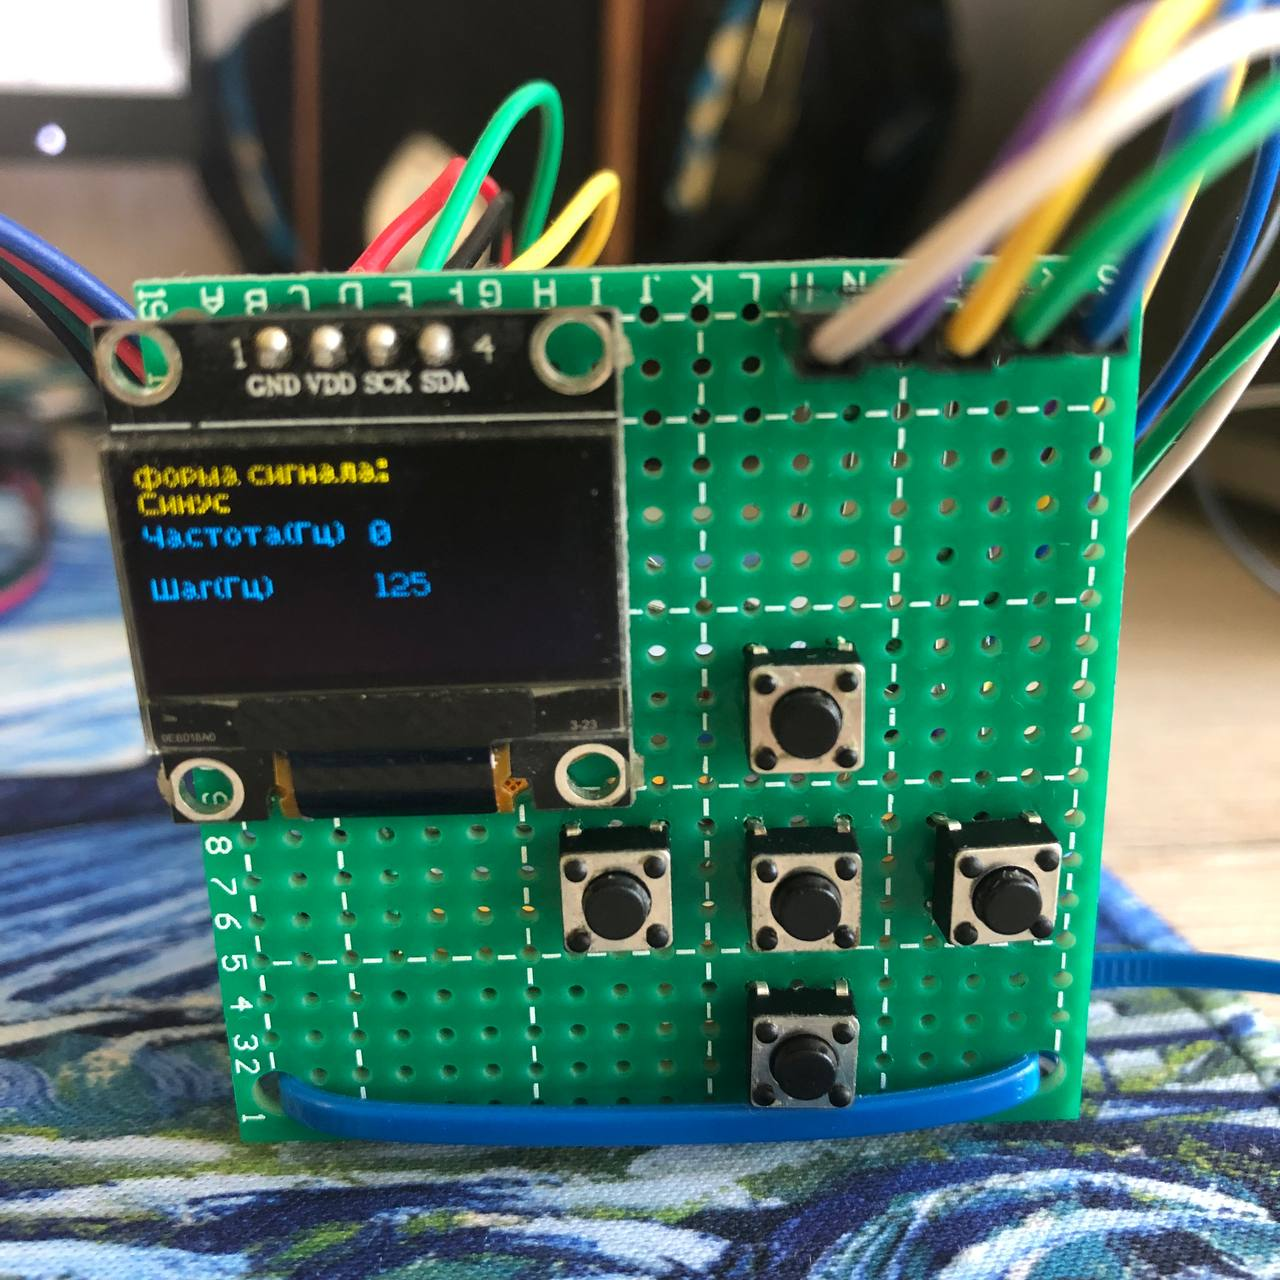
\includegraphics[width=0.8\textwidth]{../image/test1_u_st.jpg}
         \caption{Состояние устройства.}
     \end{subfigure}
     \hfill
     \begin{subfigure}[H]{0.5\textwidth}
         \centering
         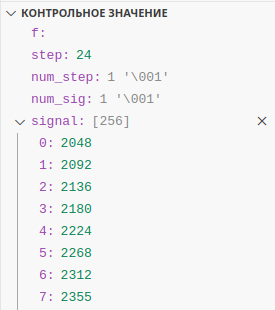
\includegraphics[width=0.725\textwidth]{../image/test1_o_st.png}
         \caption{Состояние в отладчике.}
     \end{subfigure}
        \caption{Процедура выбора шага частотой 125 Гц.}
	\end{figure}
	
	Выбор шага происходит циклично, поэтому для него требуется только одна кнопка. Самим же шагом по частоте является переменная step, которая содержит в себе для микроконтроллера код частоты, соответствующий частотам генерируемого сигнала.
	
	С помощью клавиш F- и F+ регулируется частота с заданным шагом. Возможный диапазон частот, который можно выставить 125 --- 50000 Гц. Алгоритм представлен блок-схемами (рис. 3.20).
	
	\begin{figure}[H]\captionsetup[subfigure]{font=normalsize}
     \begin{subfigure}[H]{1\textwidth}
         \centering
         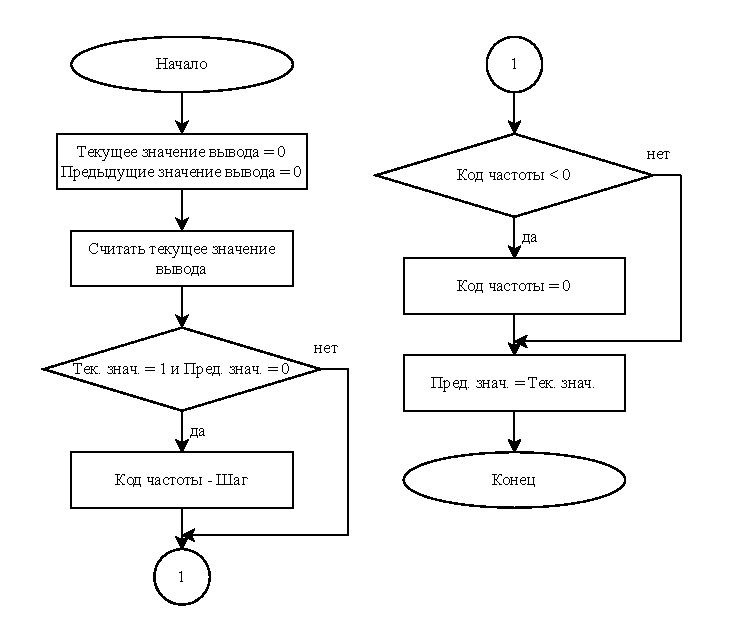
\includegraphics[width=0.775\textwidth]{../image/minus_freq.pdf}
         \caption{Блок-схема алгоритма уменьшения частоты.}
     \end{subfigure}
     \hfill
     \begin{subfigure}[H]{1\textwidth}
         \centering
         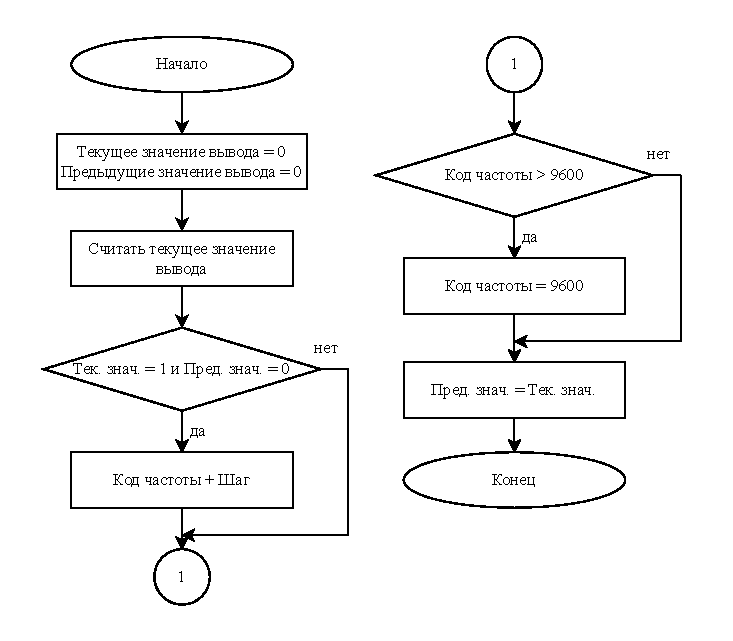
\includegraphics[width=0.775\textwidth]{../image/plus_freq.pdf}
         \caption{Блок-схема алгоритма увеличения частоты.}
     \end{subfigure}
        \caption{Блок-схемы алгоритмов регулировки частоты.}
	\end{figure}
	
	Все функции отрабатывают корректно. Выставим сигнал синуса с частотой 1875 Гц.
	
	\begin{figure}[H]\captionsetup[subfigure]{font=normalsize}
     \begin{subfigure}[H]{0.5\textwidth}
         \centering
         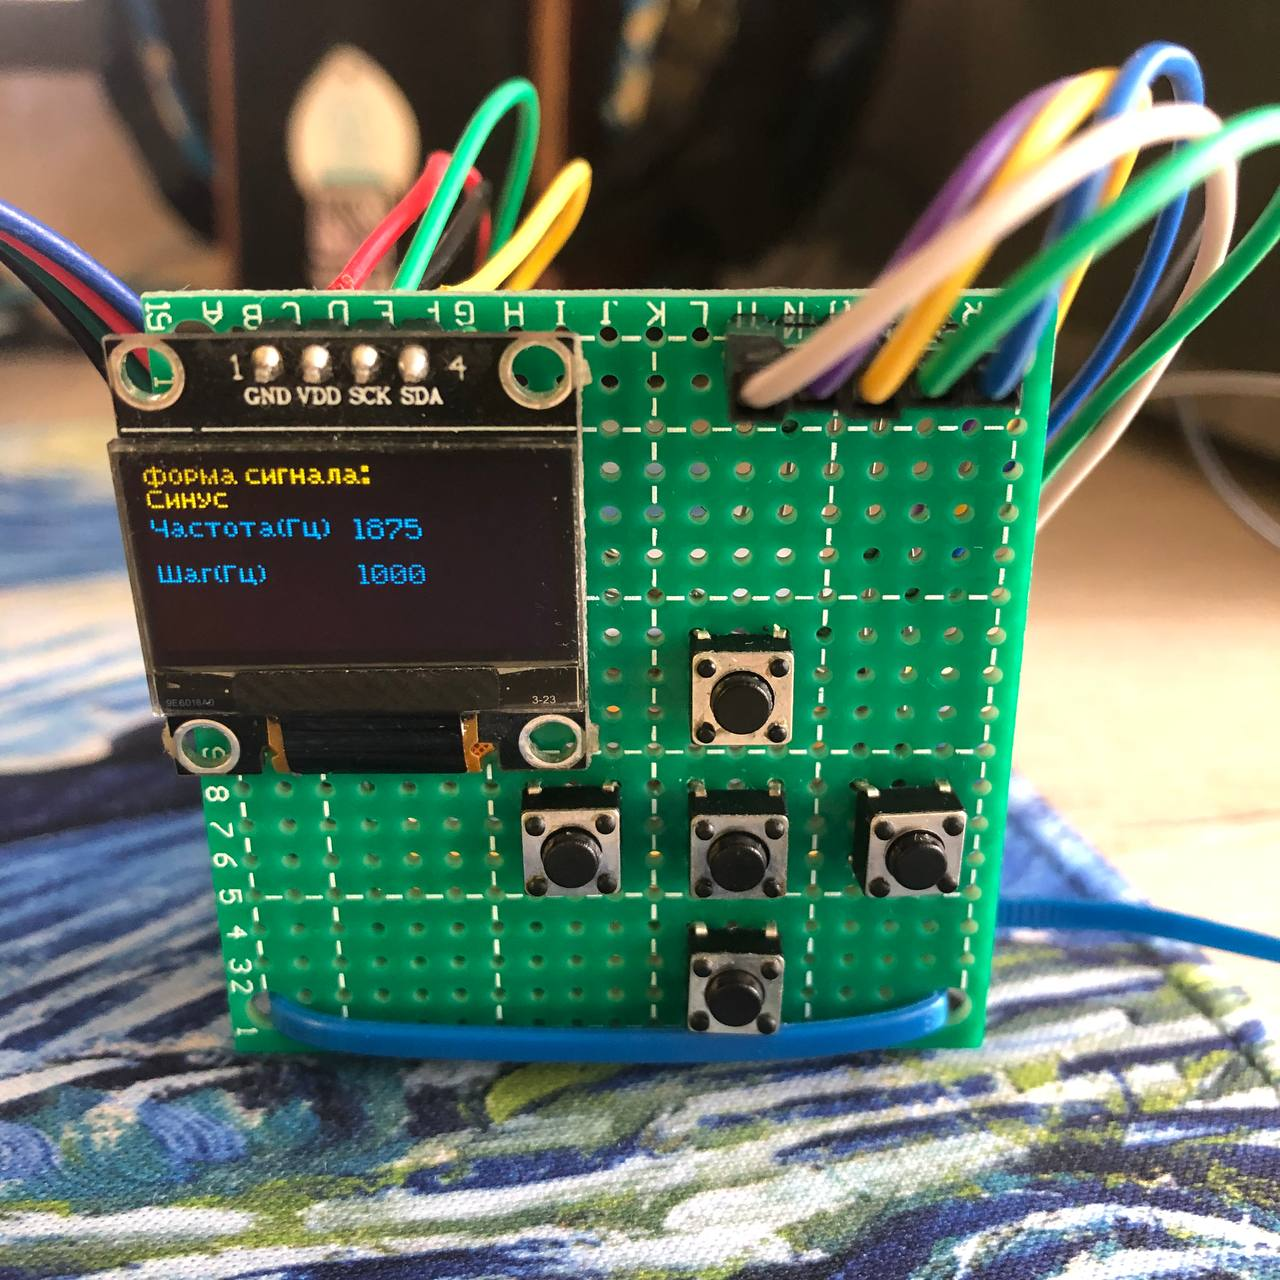
\includegraphics[width=0.7\textwidth]{../image/test4_u_f.jpg}
         \caption{Состояние устройства.}
    	\end{subfigure}
     \hfill
     \begin{subfigure}[H]{0.5\textwidth}
         \centering
         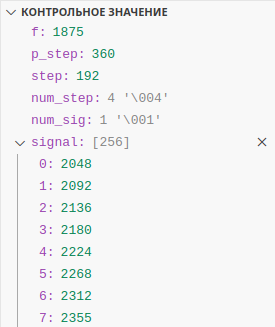
\includegraphics[width=0.62\textwidth]{../image/test4_o_f.png}
         \caption{Состояние в отладчике.}
     \end{subfigure}
        \caption{Выставленные параметры.}
	\end{figure}
	
	Снимем сигнал с осциллографа.
	\begin{figure}[H]
    \centering
    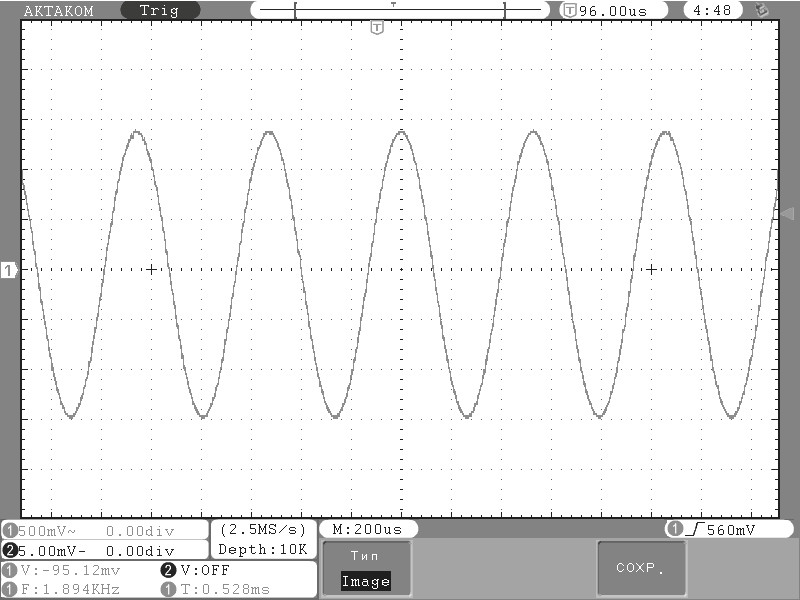
\includegraphics[width=0.75\textwidth]{../image/1875.bmp}
    \caption{Синусоидальный сигнал с частотой 1875 Гц.}
	\end{figure}	
	
	Рассмотрим все формы сигналов на частоте 1 кГц.
	
	На рис. 3.16 изображён синусоидальный сигнал с частотой 1 кГц.

	\begin{figure}[H]
    \centering
    \includegraphics[width=0.75\textwidth]{../image/sin1.bmp}
    \caption{Синусоидальный сигнал с частотой 1 кГц.}
	\end{figure}	


	На рис. 3.17 изображён прямоугольный сигнал с частотой 1 кГц.
	\begin{figure}[H]
    \centering
    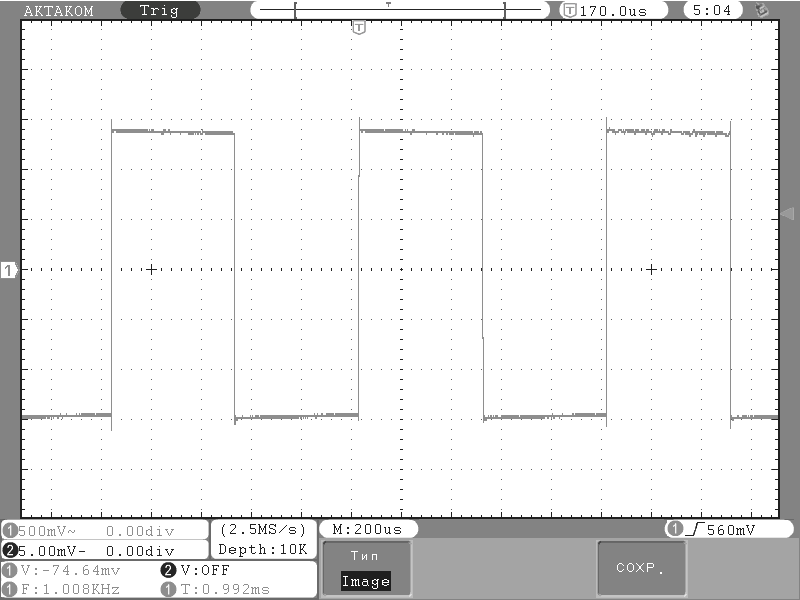
\includegraphics[width=0.75\textwidth]{../image/square1.bmp}
    \caption{Прямоугольный сигнал с частотой 1 кГц.}
	\end{figure}	
	
	На рис. 3.18 изображён треугольный сигнал с частотой 1 кГц.
	\begin{figure}[H]
    \centering
    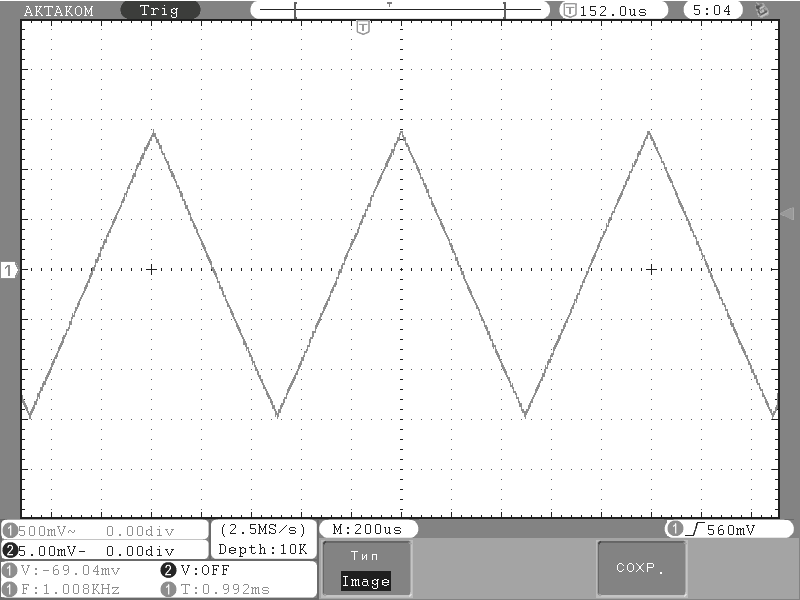
\includegraphics[width=0.75\textwidth]{../image/triangle1.bmp}
    \caption{Треугольный сигнал с частотой 1 кГц.}
	\end{figure}	

	На рис. 3.19 изображён обратный пилообразный сигнал с частотой 1 кГц.
	
	\begin{figure}[H]
    \centering
    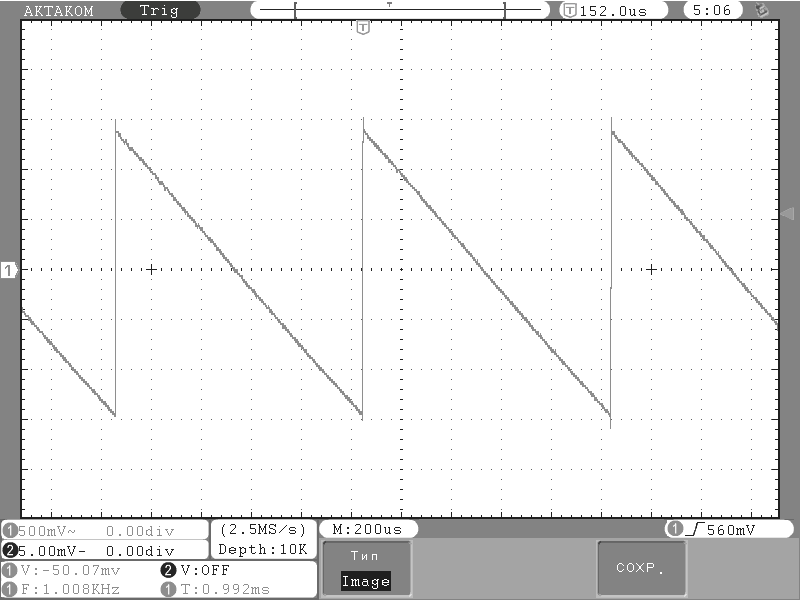
\includegraphics[width=0.75\textwidth]{../image/l_saw1.bmp}
    \caption{Обратный пилообразный сигнал с частотой 1 кГц.}
	\end{figure}	

	На рис. 3.20 изображён пилообразный сигнал с частотой 1 кГц.	
	\begin{figure}[H]
    \centering
    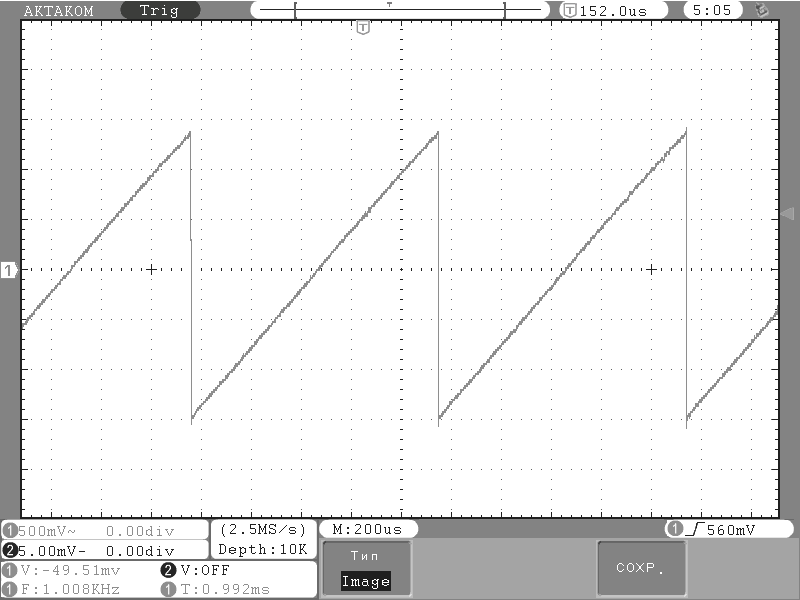
\includegraphics[width=0.75\textwidth]{../image/r_saw1.bmp}
    \caption{Пилообразный сигнал с частотой 1 кГц.}
	\end{figure}	
	
	Как можно заметить устройство генерирует все заданные формы сигналов. Рассмотрим более высокие частоты синуса (рис 3.21).
	
	\begin{figure}[H]
    \centering
    \includegraphics[width=0.75\textwidth]{../image/sin10.bmp}
    \caption{Синусоидальный сигнал с частотой 10 кГц.}
	\end{figure}	
	
	На 10 кГц уже можно наблюдать, что отсчёты сигнала не такие ровные. На 50 кГц синусоиду уже трудно узнать (рис. 3.22). На её период приходится 7 отсчётов.
	
	\begin{figure}[H]
    \centering
    \includegraphics[width=0.7\textwidth]{../image/sin50.bmp}
    \caption{Синусоидальный сигнал с частотой 50 кГц.}
	\end{figure}	
	
	Исходя из этого можно сделать вывод, что присутствует шум цифро-аналогового преобразователя. 
	
	Проведём анализ сигнала в программе GNU Octave~\cite{octave}. Возьмём записанные осциллографом отсчёты синусоидального сигнала на частоте 1 кГц и построим для сравнения такую же форму сигнала, но с заведомо большей частотой дискретизации. Будем считать построенную форму идеальным сигналом. Частота дискретизации ЦАП составляет 1 МГц, а для построения возьмём 5 МГц.
	
\begin{code}
\captionof{listing}{Сравнение сигналов}
\begin{minted}[mathescape,linenos,frame=lines,breaklines]{text}
clear all
sig = csvread('data.csv'); % сигнал с осциллографа
Td = sig(2,1)-sig(1,1); % период дискретизаци
t=linspace(0, 24999*Td, 25000); % интервал времени для идеального сигнала
f = 1000; % частота идеального сигнала
ideal_sin = -2.9 / 2 * sin(2 * pi * f * t) + 3.3 / 2 + 0.05; % идеальный сигнал
ideal_sin=ideal_sin.';
plot(t, sig(:,2), 'LineWidth', 0.5)
hold on;
plot(t, ideal_sin, 'LineWidth', 2)
xlabel('Время (с)');
ylabel('Напряжение (В)');
\end{minted}
\end{code}

	В итоге получим следующее изображение, из которого можно заметить, что сигнал с генератора не совпадает с идеальным, то есть его частота не составляет ровно 1 кГц (рис. 3.23.).
	
	\begin{figure}[H]
    \centering
    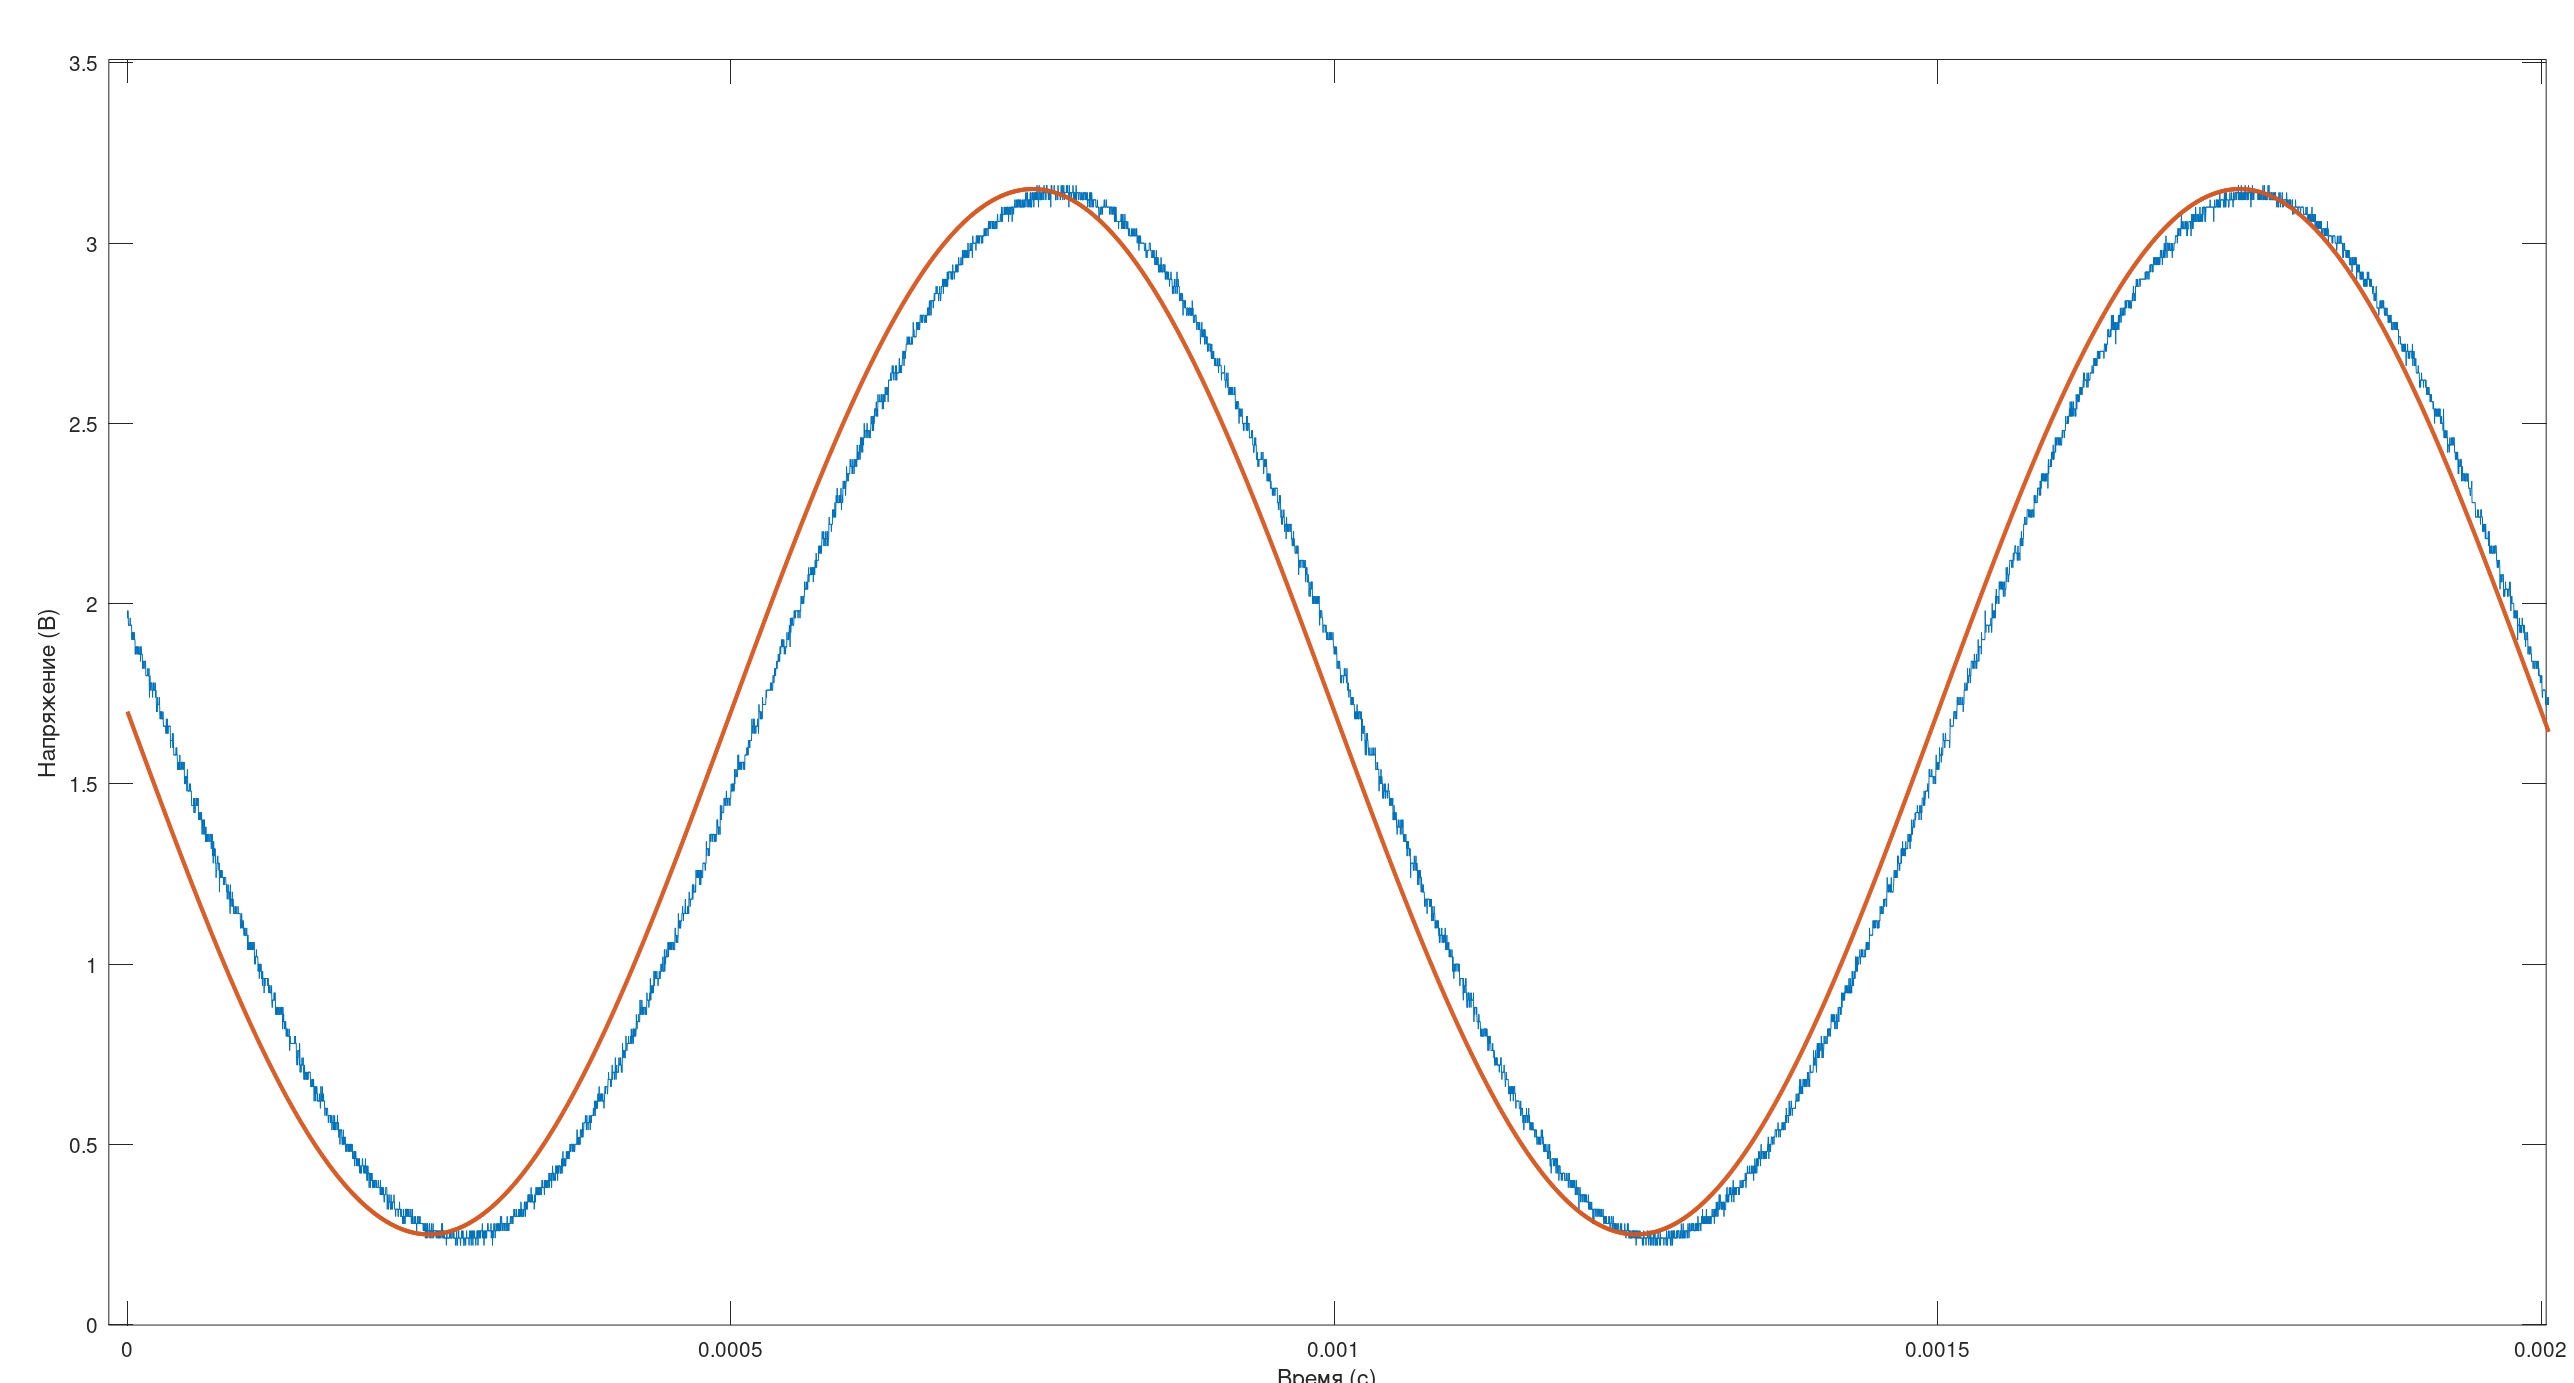
\includegraphics[width=1\textwidth]{../image/ideal.png}
    \caption{Сравнение записанного и идеального сигналов.}
	\end{figure}	
	
	Проведём спектральный анализ нашего сигнала, перейдя от временной составляющей к частотной с помощью быстрого преобразования Фурье~\cite{cos}.

\begin{code}
\captionof{listing}{Спектральный анализ}
\begin{minted}[mathescape,linenos,frame=lines,breaklines]{text}
fft_ideal = abs(fft(ideal_sin)/25000);
data_sig = sig(:, 2);
fft_sig = abs(fft(data_sig)/25000);
ff=linspace(0,24999/25000*1/Td, 1/Td/25000);
ff=ff.'

output_data_fft = zeros(length(fft_ideal), 2);
output_data_fft(:, 1) = fft_ideal;
output_data_fft(:, 2) = fft_sig;

csvwrite('fft.CSV', output_data_fft);
csvwrite('ff.CSV', ff);
\end{minted}
\end{code}
	
	На рис. 3.24 можно заметить смещение по частоте и утечку фазы.

	\begin{figure}[H]
    \centering
    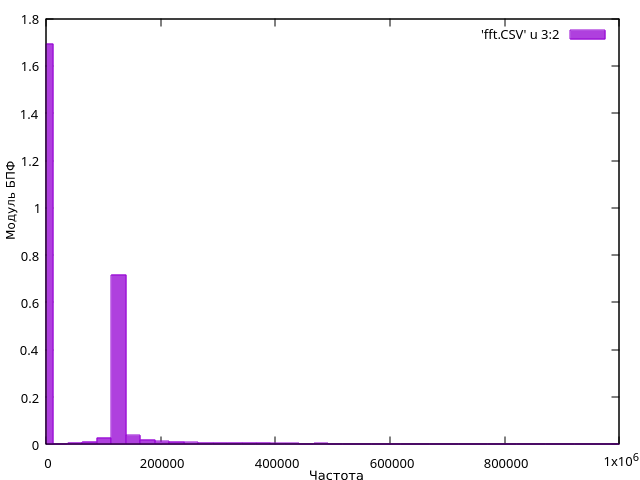
\includegraphics[width=1\textwidth]{../image/fft.png}
    \caption{Спектр сигнала.}
	\end{figure}	
	
		
	
\section{Вывод по третьей главе}
	Таким образом, генератор сигналов был реализован в виде макета. Тестирование показало, что устройство успешно выполняет заданные функции. Были проверены различные формы сигналов, а также возможность регулирования частоты с заданным шагом. Дополнительно был проведен анализ сигнала с помощью сравнения с построенным идеальным и рассмотрением спектра. 
	
	В качестве возможных усовершенствований можно рассмотреть:
	\begin{enumerate}
	\item Увеличение разрешения регулирования частоты и диапазона частот;
	\item Установка фильтра на выход цифро-аналогового преобразователя;
	\item Возможность регулировки амплитуды;
	\item Возможность регулировки фазы;
	\item Разработка печатной платы и корпуса.
	\end{enumerate}

\chapter*{ЗАКЛЮЧЕНИЕ}
	В результате выполнения данной выпускной квалификационной работы была достигнута поставленная цель --- разработан программный генератор сигналов на микроконтроллере STM32F103RCT6, позволяющий генерировать сигналы разной формы, со следующими характеристиками:

	\begin{itemize}
		\item Формы сигналов: синус, треугольник, прямоугольник, пилообразная, обратная пилообразная.
		\item Частота сигнала: 125 --- 50000 Гц.
		\item Амплитуда: 3 В.
		\item Шаг по частоте: 125, 250, 500, 1000 Гц.
	\end{itemize}

	Помимо микроконтроллера генератор состоит из дисплея с разрешением 128 на 64 пикселя, работающего по интерфейсу I2C, и пяти кнопок управления.

	Для достижения поставленной цели были выполнены все задачи, а именно:
	\begin{enumerate}
		\item Выбран метод генерации сигналов.
		\item Выбран микроконтроллер.
		\item Выбрана среда разработки.
		\item Спроектирован генератор.
		\item Сконструирован макет.
		\item Разработана и протестирована программа.
	\end{enumerate}

	Реализованный генератор сигналов отличается простотой, так как использует встроенный цифро-аналоговый преобразователь микроконтроллера и тем самым компактен, а также доступные элементы периферии ввиду этого также его плюсом является невысокая стоимость. 
\addcontentsline{toc}{chapter}{ЗАКЛЮЧЕНИЕ}




\newpage
\addcontentsline{toc}{chapter}{СПИСОК ИСПОЛЬЗОВАННОЙ ЛИТЕРАТУРЫ}
\printbibliography[title={СПИСОК ИСПОЛЬЗОВАННОЙ ЛИТЕРАТУРЫ}]

\appendix
\newpage
\addcontentsline{toc}{chapter}{Приложение 1}
\begin{flushright}
\uppercase{Приложение 1}\label{appendix1}
\end{flushright}

% Проверить работу в содержании, правильную нумерацию приложений и переброску по ссылки.
%\chapter*{Приложение A}
%\phantomsection
%\addcontentsline{toc}{chapter}{Приложение A}
%\label{appendixA}


\makelastpage
\end{document}

